%% -*- coding: utf-8; -*-

\documentclass[
  msc
]{ThesisPUC}

%%%
%%% Additional Packages
%%%

%% \usepackage[brazilian]{babel}      %% in ThesisPUC.cls
%% \usepackage[utf8]{inputenc}        %% .
%% \usepackage[T1]{fontenc}           %% .
%% \usepackage{lmodern}               %% .
%% \usepackage[pdftex]{graphicx}	%% .

\usepackage{tabularx}
\usepackage{multirow}
\usepackage{multicol}
\usepackage{colortbl}
\usepackage[%
  dvipsnames,
  svgnames,
  x11names,
  fixpdftex
]{xcolor}
\usepackage{numprint}
\usepackage{textcomp}
\usepackage{booktabs}
\usepackage{amsmath}
\usepackage{enumitem}
\usepackage{amssymb}
\usepackage{textcomp}
\usepackage{algorithm}
\usepackage{algorithmic}

%\usepackage{etoolbox}

\DeclareGraphicsExtensions{.png, .pdf}

%% numprint 
\npthousandsep{.}
\npdecimalsign{,}

%% ThesisPUC option
%% \tablesmode{figtab} %% [nada, fig, tab ou figtab]


%%%
%%% Counters
%%%

%% uncomment and change for other depth values
%% \setcounter{tocdepth}{3}
%% \setcounter{lofdepth}{3}
%% \setcounter{lotdepth}{3}
%% \setcounter{secnumdepth}{3}


%%%
%%% New commands and other global definitions
%%%

% -*- coding: iso-8859-1; -*-

%%%
%%% Newcommands
%%%

\newcommand{\degree}{\ensuremath{^\circ}}

\newcommand{\cetem}{Centro de Tecnologia Mineral}

\newcommand{\mybulletOB}{%
  % \textbullet
  % \checkmark
  $\triangleright$
  %\textopenbullet
}

\newcolumntype{L}{>{\raggedright \arraybackslash}X}
\newcolumntype{R}{>{\raggedleft \arraybackslash}X}
\newcolumntype{C}{>{\centering \arraybackslash}X}
\newcolumntype{M}[1]{>{\centering\hspace{0pt}}m{#1}}

\newcommand{\mrcel}[2]{%
\begin{tabular}[c]{@{}c@{}}#1\\#2\end{tabular}}

\newcommand{\mrcell}[2]{%
\begin{tabular}[l]{@{}l@{}}#1\\#2\end{tabular}}

\newcommand{\mrcelthree}[3]{%
\begin{tabular}[c]{@{}c@{}c@{}}#1\\#2\\#3\end{tabular}}

\newcommand{\mrcelcolorg}[2]{%
\begin{tabular}{l}\rowcolor{Gainsboro}#1\\#2\end{tabular}}

\newcommand{\mytbcimg}[3]{%
  \multicolumn{1}{C}{\parbox[c]{#1}{\includegraphics[width=#2]{#3}}}}


%%%
%%% Abreviation Title
%%%

%% \abreviationstitle{Lista de Abreviaturas}
%% \abreviationstitleuk{List of Abreviations}


%%%
%%% Misc.
%%%

\usecolour{true}


%%%
%%% Titulos
%%%

\author{Daniel Lemes Gribel}
\authorR{Lemes Gribel, Daniel}

\adviser{Thibaut Vidal}{Dr.}
\adviserR{Vidal, Thibaut}

%\coadviser{Otávio da Fonseca Martins Gomes}{Dr.}
%\coadviserR{da Fonseca Martins Gomes, Otávio}
%\coadviserInst{Centro de Tecnologia Mineral}{CETEM/MCTI}

\title{Meta-heuristics for data clustering}

%\titleuk{Meta-heuristics for data clustering}

%% \subtitulo{Aqui vai o subtitulo caso precise}

\day{$1^{st}$}
\month{March}
\year{2017}

\city{Rio de Janeiro}
\CDD{620.11}
\department{Informática}
\program{Informática}
\school{Centro Técnico Científico}
\university{Pontifícia Universidade Católica do Rio de Janeiro}
\uni{PUC-Rio}


%%%
%%% Jury
%%%

\jury{%
  \jurymember{Paulo Roberto Gomes Brandão}{Prof.}
    {Universidade Federal de Minas Gerais}{UFMG}
  \jurymember{Leonardo Evangelista Lagoeiro}{Prof.}
    {Universidade Federal de Ouro Preto}{UFOP}
  \jurymember{Reiner Neumann}{Dr.}
    {Centro de Tecnologia Mineral}{CETEM/MCTI}
  \jurymember{Marcos Henrique de Pinho Maurício}{Dr.}
    {Departamento de Engenharia de Materiais}{PUC-Rio}
  \schoolhead{José Eugenio Leal}{Prof.}
}


%%%
%%% Resume
%%%

\resume{%
Obtained a bachelor’s degree in Information Systems
from the Federal University of Rio de Janeiro State
(Unirio, Rio de Janeiro, Brazil). He earned a
scholarship from CNPq in his Masters at PUC-Rio.}


%%%
%%% Acknowledgment
%%%

\acknowledgment{%
  \noindent Em primeiro lugar, gostaria de agradecer especialmente a meu
  orientador ...
  \bigskip

  \noindent Em segundo lugar ...
}


%%%
%%% Catalog prekeywords
%%%

\catalogprekeywords{%
  \catalogprekey{Informática}%
}


%%%
%%% Keywords
%%%

\keywordsuk{%
  \key{Clustering;}
  \key{Meta-heuristic;}
  \key{Unsupervised learning;}
  \key{Minimum sum-of-squares;}
  \key{Data mining;}
  \key{Combinatorial optimization.}
}

\keywords{%
  \key{Clusterização;}
  \key{Meta-heurística;}
  \key{Aprendizado não-supervisionado;}
  \key{Mínima soma dos quadrados;}
  \key{Mineração de dados;}
  \key{Otimização combinatória.}
}


%%%
%%% Abstract
%%%

\abstractuk{%
  Iron ore is a polycrystalline material created by complex natural
  processes during geological periods, which give rise to ...
}
  
\abstract{%
  O minério de ferro é um material policristalino oriundo de processos
  naturais complexos durante tempos geológicos, que dão origem ...
}

\begin{document}

  %%% -*- coding: utf-8; -*-
\begin{thenotations}

  \noindent
  \begin{tabular}{ll}
    MSSC -- Minimum sum-of-squares clustering\\
    GA -- Genetic algorithm\\
  \end{tabular}
  
\end{thenotations}

  % -*- coding: utf-8; -*-

\chapter{Introduction}

This is the first chapter...

In this chapter, let's have a nice image:

\begin{figure} [h]
  \begin{center}
    \includegraphics[height=243pt,width=400pt]{images/fig2-6}
    \caption{Exemplo de limiarização pentamodal: (a) Imagem original
      em 256 tons de cinza; (b) Imagem quinária com as fases
      diferençadas com cores; (c) Tons de corte no
      histograma.\cite{74}}\label{fig:2-6}
  \end{center}
\end{figure}

  % -*- coding: utf-8; -*-
\chapter{Problem Statement and Literature Review}

Most algorithms proposed for data clustering are based on heuristics with intuitive procedures \cite{Fraley2002}. These algorithms are also referred as ad-hoc methods, once they are solutions designed for specific clustering criteria, being non-generalizable and not adaptive. As these ad-hoc methods are based on greedy constructions or local improvements, they have some limitation regarding solution quality and local optimum convergence.

There is little systematic guidance in such algorithms for solving important questions in cluster analysis \cite{Fraley2002}. K-means is an example of a very popular ad-hoc algorithm for clustering, based on iterative updates of cluster centers until convergence. Although k-means is easy to implement and usually demand low computational time, it has not any optimality guarantee and is highly dependent on initial conditions to deliver good outcomes.

However, in the recent years there has been a considerable growth of clustering methods designed in a model-oriented way. This approach is based on formal models that usually produce more accurate solutions than ad-hoc methods as they clearly state an objective to be achieved.

\section{Ad-hoc methods}
The ad-hoc methods proposed for data clustering usually belong to two large classes: hierarchical and partitional algorithms.

% Hierarchical clustering
Hierarchical clustering works by successively agglomerating or separating clusters at each stage according to some distance measure. The methods of this class can be roughly separated into two groups: agglomerative and divisive methods. In an agglomerative approach, each data point starts at its own cluster and at each stage of the algorithm it joins the two most similar clusters, until a single cluster containing all data points is reached. The divisive method is the opposite. The method proceeds by separating $n$ data points successively into finer groups. 

Several algorithms for data clustering are based on hierarchical constructions, once they do not require the number of clusters a priori and are independent from initial conditions, as strategic starting points. However, hierarchical methods are computationally expensive -- usually O($n^2$ log $n$) for computational complexity -- and all decisions about joining/separating sets of points are definitive, i.e., it is impossible to revert any merge or split operation. BIRCH (Balanced Iterative Reducing and Clustering Using Hierarchies) \cite{Zhang96} and CURE (Clustering Using Representatives) \cite{Guha1998} are examples of popular hierarchical clustering algorithms.
 
%\subsubsection{Partitional clustering}
The methods belonging to partitional clustering directly divides data points into some pre-specified number of clusters without any hierarchical structure \cite{Xu2005}. It is composed by methods based on iterative relocation of data points between clusters that, at each iteration, reduce the value of some criteria function until convergence \cite{Karkkainen2006}. The minimum sum-of-squares function is one of the most widely used criteria, which aims to minimize the sum of each data point to the center of its cluster. K-means and PAM (Partitioning Around Medoids) are quite widespread partitioning clustering methods. Although partitional clustering algorithms are suitable for large data sets due to efficiency in computational time, they require the number of clusters in advance and are heavily dependent on the initial conditions, which can lead algorithms like k-means to a premature convergence \cite{Das2009}.

\section{Model-driven clustering}
The above classes of ad-hoc methods are not guided by a model, but by iterative constructions or re-assignments according to some underlying criteria. For instance, in K-means algorithm, the criteria is to assign data points to the closest center after the calculation of centers position. In hierarchical methods, the criteria to merge/split a solution is based on a distance metric between pairs of clusters. Due to these characteristics, it is difficult to assess if erratic results come from inappropriate methods, or from a data that does not intuitively leads to the result that we desire.

In order to detect this kind of behaviour, some solutions have been designed to face data clustering from a model-oriented perspective, which means giving a formal definition of the clustering problem as an optimization problem, where clear objective functions and restrictions are set. Therefore, one can apply a method that minimizes/maximizes an objective function to solve the model.

The work of Hansen and Jaumard \cite{Hansen1997} states that most of clustering tasks are composed by the following elements:

\begin{itemize}

	\item \textit{Data}. Observation of $d$ characteristics in $n$ entities (patterns). This yields a $n \times d$ data matrix.

	\item \textit{Similarities}. Computation of the similarities between entities, i.e., the derived measures from features that indicates how similar (dissimilar) are each pair of entities.

	\item \textit{Constraints}. Specification of existing constraints in the clustering task. For instance: number of clusters, maximum cardinality per cluster, number of clusters an entity can be assigned to, etc.

	\item \textit{Criterion}. Selection of the criterion to express homogeneity or separability of the clusters.

	\item \textit{Algorithm}. Design of the algorithm to solve the clustering problem.

	\item \textit{Interpretation}. Analysis on how meaningful are the generated clusters. For instance: use of descriptive statistics and data mining indicators.

\end{itemize}

Except for \textit{Interpretation}, the above steps that characterize a general clustering task are profitably addressed by the mathematical programming perspective, as it is capable of explicitly define and delimit the problem.

In this work, we treat the clustering task as an optimization problem, where we can achieve near optimality regarding a specific objective. Thus, we consider a particular formulation for data clustering, the Minimum sum-of-squares clustering (MSSC). Many formulations can be done to express a clustering task. Besides that, some optimization problems are more suitable for specific clustering tasks, or specific data sets.

\section{The MSSC problem}
The MSSC problem -- also referred as the \textit{discrete clustering} problem or the \textit{hard clustering} problem -- has been extensively studied in the literature for data clustering, possibly because this is the natural model which is addressed by the k-means algorithm. It was first formulated mathematically by Vinod \cite{Vinod1969}, where the MSSC is defined as a problem that assumes integer variables that can take values 0 or 1 only, recognizing it as an Integer programming problem.

In the MSSC problem we aim to minimize the total sum of the distances of each data point to the mean point in its cluster. We are given set $X$ of $n$ data points in a $d$-dimensional space $\mathbb{R}^d$ \cite{Bagirov2006}:

\begin{center}%
$X = \{x_1, x_2, ..., x_n\}$, where $x_i \in \mathbb{R}^d, \quad i = 1, ..., n.$
\end{center}

Then, if we consider $S$ as the set of all possible subsets obtained from elements in $X$, the clustering procedure must generate a partition $\bar{S}$ of $S$ with $m$ subsets $S_k \in S (S_k \neq \emptyset)$, where $m$ is the number of desired clusters and $k = \{1,...,\left | S \right |\}$. In other words, a clustering algorithm aims to generate a partition that groups data consistently, with most similar data points belonging to the same group and dissimilar data points belonging to different groups.

In order to define the similarity between two data points in the space, a function $d$ assigns to any pair $x, y \in \mathbb{R}^d$ a distance metric $d(x,y) \in \mathbb{R}$. Many distance measures could be used to characterize how similar two data points or patterns are. A popular one in the domain of data mining is the Euclidean distance, that can often be used to reflect the similarity between two patterns when considering multiple dimensions (features) \cite{Jain1999}:
%The assignment is done in such a way that the greater is the similarity (proximity) within a cluster and the greater is the difference between clusters, the better is the clustering.

\begin{equation}
\label{euclidean}
d(x,y) = \sqrt{\sum_{q=1}^{d}(x_{q} - y_{q})^2} = \left \| x - y \right \|, \quad x, y \in \mathbb{R}^d
\end{equation}

Here, $x_{q}$ is the value of the $q$-th feature of a data point $x$, $d$ is the number of features and $q = \{1,...,d\}$. Analogously, the set of data points $x_i \in X$ can be described as a matrix $X'_{n \times d}$, where an entry $x_{iq}$ is the value of the $q$-th feature for the $i$-th data point. In this work we consider that the data points (including the centroids) are in the Euclidean space, so the measure above (\ref{euclidean}) is used to express the distance between any two points. Therefore, the MSSC problem can be formulated as the following set partitioning problem:

\begin{equation} \label{eq:of}
\textrm{Minimize} \sum_{k=1}^{\left | S \right |}z_k y_k
\end{equation}

\begin{equation}
\sum_{k=1}^{\left | S \right |}a_{ik}y_k = 1, \quad \forall i
\end{equation}

\begin{equation}
\sum_{k=1}^{\left | S \right |}y_k = m
\end{equation}

\begin{equation}
a_{ik} \in \{0,1\}, \quad \forall i,k
\end{equation}

\begin{equation}
y_k \in \{0,1\}, \quad \forall k
\end{equation}

\noindent where $\left | S \right |$ is the size of the set $S$; $a_{ik} = 1$ if $x_i \in S_k$ and $a_{ik} = 0$ otherwise; $y_k$ are the decision variables, with $y_k = 1$ if the subset $S_k$ is chosen ($S_k \in \bar{S}$) and $y_k = 0$ otherwise; and $z_k$ is the cost function on subset $S_k$, i.e., the cost within the $k$-th subset. In the MSSC problem, the centroid is the mean point $c_k$ of cluster $S_k$. Thus, the contribution $z_k$ of each subset to the objective function is:
	\begin{equation}
	z_k = \sum_{x_i \in S_k} d(x_i, c_k)
	\end{equation}
	\begin{center}
	where $c_k = $ \Large $\frac{\sum_{i = 1}^{n}a_{ik}x_i}{\sum_{i = 1}^{n}a_{ik}}$	
	\end{center}
	
\subsection{Computational complexity}
Regarding computational complexity, the MSSC can be solved in $O(n^3)$ time for $m \geq 2$ and one dimensional data \cite{Spath1980}. For $m \geq 2$ and general dimension, the MSSC is NP-hard \cite{Aloise2009}. If both $m$ and $d$ are fixed, the problem can be solved in $O(n^{md+1})$ time \cite{Inaba1994}, which may be very time-consuming. However, the hardness of MSSC is not measured only by the number of points (samples), dimensions and clusters, it also depends on the distribution of points \cite{Aloise2009Branch}.

\noindent [TO-DO] complete with the explanation why complexity depends on points distribution

\subsection{Solution techniques}
Many solution techniques have been developed in recent years to solve the MSSC problem. These techniques can be separated into different categories, based on their exact or heuristic nature, whether they are deterministic or probabilistic, whether they process complete solutions or construct solutions during the search, and finally whether they maintain a single candidate solution or have a population of solutions \cite{Das2009}. This range of methods includes construction methods and local searches, which aims to repeatedly seek for better solutions according to some fitness; meta-heuristic algorithms; and mathematical programming techniques. In this section, we review some techniques and previous works that have been designed for the resolution of the MSSC problem.

Hansen \cite{Hansen2001} proposed a local search called J-MEANS for the MSSC problem. The neighbourhood of a current solution is defined by all possible centroid-to-object relocations followed by corresponding changes of assignments. Thus, a move in J-MEANS corresponds to replacing an existing centroid $x_i$ by a data point $x_j$. The move is done by selecting the pair of indices ($i$, $j$) that brings the highest gain in the objective function. Finally, the centroid $x_i$ is replaced by $x_j$ and the corresponding assignment updates are done. Moves are made in these neighbourhoods whenever the value of a neighbour's objective function is better than the current solution, until a local optimum is reached. As the J-MEANS is a general local search, it is also applied to fit into meta-heuristics as the Variable Neighbourhood Search (VNS). The J-MEANS local search seems to work well in some problem instances where the number of clusters is large, so that data points could be centroids of some clusters in the current solution.

Recently, different incremental algorithms have been developed to address the choice of initial solutions in the k-means algorithm. Incremental clustering algorithms start from an initial solution with $k - 1$ centers for the ($k - 1$)-clustering problem and attempt to optimally add one new cluster by placing the $k-$th center in an appropriate position. The global k-means \cite{Likas2003} is an incremental algorithm that solves the MSSC problem by considering each data point as a candidate for the $k-$th cluster center.

A modified version of the global k-means (MGKM) proposed by \cite{Bagirov2008} tackles the MSSC by producing initial solutions through the resolution of an auxiliary clustering problem, rather then testing all data points as candidate centers. Experimental results demonstrate that MGKM is able to find better solutions than the global k-means, although it requires more computational effort.
 
The work of Ordin and Bagirov \cite{Ordin2014} considered the MSSC as a global optimization problem and introduced a new algorithm to improve the accuracy of MGKM. The method is an adaptation of MGKM that produces a set of initial solutions that undergo k-means, rather than considering only one initial solution at each k-means stage. The proposed method was applied on 16 real-world data sets and experiments shown that it is more accurate than MGKM.

More recently, \cite{Bagirov2016} presented an incremental algorithm based on the difference of convex representations for solving the MSSC problem, where a method is designed to solve non-smooth optimization problems at each iteration of the incremental algorithm. Large data sets ranging from tens to hundreds of thousands data points are used, and results show that this approach is efficient for solving large data sets when compared to previous incremental algorithms like MGKM and global k-means.

Many authors proposed some hybrid methods, that combine both classical algorithms with meta-heuristics. \cite{Krishna1999} and \cite{Lu2004} uses k-means as a search operator inside a genetic algorithm (GA) on the MSSC problem, in such a way that each GA candidate solution is used as a starting point for k-means. Thus, k-means assumes the role of a local search inside a broader optimization process guided by the GA.

The work of Festa \cite{Festa2013} has also treated the MSSC problem with emphasis on combinatorial optimization perspective. The proposed approach considers a biased random-key genetic algorithm (BRKGA), which was applied to biological data clustering. In random-key genetic algorithm (RKGA), candidate solutions are represented as vectors of randomly generated real numbers in the interval (0, 1]. Each vector can thus be associated to a solution in the combinatorial optimization problem, for which an objective value or fitness can be computed. To evolve the population of solutions, additional individuals are produced in order to complete the new population. This is done by crossing parent solutions. The fundamental difference between BRKGA and RKGA resides in the way parents are selected for crossing. RKGA uses any two solutions to produce a child individual, once BRKGA crosses a elite solution (good regarding fitness) with a non-elite to produce a child.

%\subsection{Construction and local search}

%\subsection{Meta-heuristics}

%\subsection{Mathematical programming methods}
  \chapter{Proposed Methodology}
\label{chap:methodology}
This chapter describes the proposed meta-heuristic to solve the MSSC problem. The designed method is based on a genetic algorithm (GA) with local improvements combined with mechanisms that allow the diversification of the population (local minima escape) and the propagation of good solutions. In this method, the local improvement procedure is performed via the running of the k-means algorithm, which takes one candidate solution in the GA population as a starting point. In other words, the method may be defined as a multi-start k-means inside a GA framework, which in turn is guided by the MSSC objective. 

\section{General structure}
\label{sec:general-structure}
The GA here proposed works through the following simple cycle of stages:

\begin{enumerate}
	\item Creation of an initial population of individuals (candidate solutions);

	\item Selection of parents individuals;

	\item Genetic manipulation to create new individuals (crossover and mutation);
	
	\item Enhancement of the produced individual (local improvement);
	
	\item Selection of survivors individuals for propagation.
	
\end{enumerate}

This general scheme of the meta-heuristic is described in more details by algorithm \ref{genetic-algo}. Initially, the method generates a random population of individuals (see \ref{sec:initial-population}). A population is a set of solutions, where each individual represents a point in a search space of the optimization problem. Then, it applies successively a number of operators to evolve this population. Firstly, it selects two parent individuals (see \ref{subsec:selection}) from the population and combines them by a crossover procedure (see \ref{subsec:crossover}), yielding to a new individual (offspring) that is added to the population. Secondly, the offspring is mutated (see \ref{subsec:mutation}) and enhanced by a local improvement (see \ref{subsec:local-improvement}), generating a new individual solution that is also added to the population. These two steps -- crossover and mutation with enhancement -- are performed many times until a termination criteria is reached.

In addition to the genetic operators mentioned above, a mechanism to select the survivor individuals is applied when a pre-defined criteria is reached (see \ref{sec:population-management}). This mechanism allows the method to propagate the best individuals and keep the diversification of the population. The following sub-sections describes how these operators and mechanisms to evolve and manage the population of solutions work.

\begin{algorithm}[!h]
\caption{Genetic algorithm framework}
\label{genetic-algo}
\begin{algorithmic}[1]
\STATE Initialize population
\WHILE{number of iterations without improvement $< I_{S}$ and $I_{max}$ not reached}
\STATE Select parents $p_1$ and $p_2$
\STATE Generate an offspring $\theta$ from $p_1$ and $p_2$ (crossover)
\STATE Generate an individual $\theta'$ by mutating $\theta$ (mutation)
\STATE Apply local improvement on $\theta'$
\STATE Add $\theta$ and $\theta'$ to the population
\IF{population size is equal to the maximum size $\Pi$ of population}
\STATE Select survivors
%\IF{best solution not improved for $I_D$ iterations}
%\STATE Diversify population
%\ENDIF
\ENDIF
\ENDWHILE
\STATE Return best solution
\end{algorithmic}
\end{algorithm}

\section{Solution representation}
\label{sec:solution-representation}
A solution (clustering partition) is represented by two direct encodings: i) the point-cluster assignment and ii) the centroids description. The idea of the point-cluster assignment is to use a genetic encoding that allocates directly $n$ data points to $m$ clusters, such that each candidate solution consists of a $n$-vector ($n$ genes) with integer values in the interval [1, $m$]. Thus, for $n$ = 4 and $m$ = 3, the encoding (1,1,3,2) allocates the first and the second data points to cluster 1; the third data point to cluster 3 and the fourth data point to cluster 2, generating the partition (\{1,2\}, \{3\}, \{4\}).

\begin{figure}[h]
  \begin{center}
    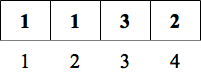
\includegraphics[width=0.3\textwidth]{img/assignment-encoding}
    \caption{Assignment encoding for $n$ = 4 and $m$ = 3}\label{fig:assignment-encoding}
  \end{center}
\end{figure}

The encoding based on the centroids description defines a solution through the feature vectors existing in each centroid. A solution is represented by a matrix $C$ of size $m \times d$, where $m$ is the number of centroids (clusters), $d$ is the number of features and an entry $c_{ij}$ of $C$ is the value of the $j$-th feature of the $i$-th centroid ($i$ = 1 ... $m$; $j$ = 1 ... $d$) (see figure \ref{fig:centroids-encoding}).

\begin{figure}[h]
  \begin{center}
    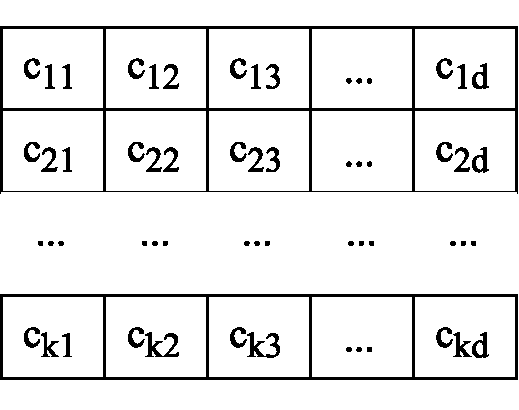
\includegraphics[width=0.4\textwidth]{img/centroids-encoding}
    \caption{Encoding based on centroids features}\label{fig:centroids-encoding}
  \end{center}
\end{figure}

\section{Initial population}
\label{sec:initial-population}
The first step in a GA is the generation of an initial population. It has been recognized that if the initial population of the GA is good, then the algorithm has a better possibility of finding a good solution \cite{Burke2004, Zitzler2000}. In this work, the initial population is randomly generated, by assigning each data point to a cluster according to a discrete uniform distribution, i.e., where each outcome is equally likely to happen. To compose the initial population, 100 individuals are created. Then, each initial individual is submitted to the local improvement. Some factors can influence the initial population or should be taken into account when an initial population is generated randomly: the search space, the fitness function, the diversity, and the number of individuals \cite{DiazGomez2007}.

\section{Individuals management}
\label{individuals-management}
In order to increase the population and start the competitive process of evolution we need to keep introducing new individuals. The generation of a new individual (offspring) begins with the random selection of two parents, $p_1$ and $p_2$, which are submitted to a crossover procedure that generates a child individual $\theta$. Then, $\theta$ is added to the population. As highly fit solutions have more chances to be selected for reproduction, the offspring -- which combines characteristics from each parent -- is likely to have a good fitness. Thus, we also consider the mutation operator, which generates a new individual $\theta'$ that is similar to $\theta$ and tends to be good regarding the fitness.

\subsection{Selection}
\label{subsec:selection}
The selection is the stage where individuals from the population are chosen to mate and generate a new individual. Due to the evolutionary behaviour of GA, the most likely individuals to be chosen for selection are the ones with good fitness. That way, the good fragments of solutions can be propagated to generate good children solutions. In the proposed method, the parent selection is done through a \textit{w}-tournament, which randomly selects $w$ individuals (in a discrete uniform distribution) from the population and keeps the one with the best fitness among the $w$ individuals to set the first parent. The fitness here considered is the value of the objective function (cost) of a solution. Then, the same selection scheme is performed to set the second parent. The value of $w$ was chosen according to a calibration process described in section \ref{sec:calibration}.

\subsection{Crossover}
\label{subsec:crossover}
Once parent solutions $p_1$ and $p_2$ were selected, they are submitted to a crossover procedure in order to produce a offspring (child) solution from them. The crossover operator works as follows:

\begin{enumerate}
	%\item Firstly, the minimum bipartite matching between centroids of $p_1$ and $p_2$ is found. Given a graph $G = (V_1, V_2, E)$, where $V_1$ is the set of centroids (nodes) of parent $p_1$, $V_2$ is the set of centroids of parent $p_2$, and $c_{ij} \in E$ is the euclidean distance for every $i \in V_1$ and $j \in V_2$; the goal is to find a one-to-one matching $M$ such that the sum of the values of the edges in $M$ is minimum. In other words, the goal is to produce the one-to-one assignment of centroids from different sets (parents), in such a way that the sum of all distances considered in the assignment is minimized. This matching problem is solved by the Hungarian method \cite{Kuhn1955} and leads to $m$ pairs of centroids, where $m$ is the number of clusters (centroids).

	\item Firstly, a solution for the minimum weighted bipartite matching between centroids of $p_1$ and $p_2$ is found (figure \ref{fig:crossover} (b)). Finding such a matching is known as the assignment problem. Let $G = (V, E)$ be a complete bipartite graph whose node set can be partitioned as $V = X \cup Y$, with the property that every edge $e \in E$ has one end in $X$ and the other in $Y$, and every node of $X$ is connected to every node of $Y$. Consider also that $|X| = |Y| = m$. An assignment $M$ in $G$ is the subset of edges $M \subseteq E$ of minimum cost, such that each node appears in exactly one edge in $M$ \cite{tardos}. In our case, the nodes in $X$ and $Y$ correspond to the centroids of $p_1$ and $p_2$, respectively. The cost of an edge $e \in E$ is the euclidean distance between two centroids $c' \in X$ and $c'' \in Y$. Thus, the goal is to produce the one-to-one assignment of centroids from different sets (parents), in such a way that the sum of all distances considered in the assignment is minimized. In other words, we aim to join the similar centroids of different individuals. This matching problem is solved by the Hungarian method \cite{Kuhn1955} and leads to $m$ pairs of centroids, where $m$ is the number of clusters (centroids).

%One set of nodes in the matching problem is composed by the centroids of $p_1$ and the other set is composed by the centroids of $p_2$. The goal is to produce the one-to-one assignment of centroids from different sets, in such a way that the overall edges weight (distances) is minimized.

	\item For each pair of centroids resulted from the assignment solution, one of them is randomly selected (figure \ref{fig:crossover} (c)) and set as a centroid of the offspring, resulting in a solution with $m$ centroids, each coming from $p_1$ or $p_2$ (figure \ref{fig:crossover} (d)).

	\item Finally, data points are assigned to the closest offspring centroid.
\end{enumerate}

\begin{figure}[H]
  \begin{center}
    
\includegraphics[width=1.0\textwidth]{img/crossover}
    \caption{Crossover based on centroids matching: (a) two parent solutions; (b) the assignment between centroids of $p_1$ and $p_2$; (c) random selection of matched centroids and (d) the produced offspring.}\label{fig:crossover}
  \end{center}
\end{figure}

%Given a graph $G = (V_1 \union V_2, E)$, where $V_1$ is the set of centroids (nodes) of parent $p_1$, $V_2$ is the set of centroids of parent $p_2$, and an edge $e_{ij} \in E$ is the euclidean distance between a centroid $c_i \in V_1$ and a centroid $c_j \in V_2$; the minimum matching in this case is the one-to-one assignment of centroids $c_i \in V_1$ to centroids $c_j \in V_2$, in such a way that the sum of the weights of $e'_{ij}$ in the assignment is minimum. 

%A Bipartite Graph G = (V, E) is a graph in which the vertex set V is divided into two disjoint subsets V_1 and V_2, such that every edge e \in E has one end point in V_1 and the other end point in V_2. Here, V_1 contains all centroids of p_1 and V_2 contains all centroids of p_2. Thus, |V_1| = |V_2|. That is it, among the |V|^2 candidate edges to be chosen, we have to select |V| edges such that every node is connected and every edge e \in E has one end point in V_1 and the other end point in V_2.

%In other words, we aim to connect the most similar nodes that are in different sets.

\subsection{Mutation}
\label{subsec:mutation}
The use of mutation is typically motivated by the possible permanent loss of genetic material during the execution of a GA. It is possible that after several generations performing the selection followed by crossover a specific genetic material (fragment) in all solutions of the population is led to the same value. If this happens, selection and crossover will not be able to restore the lost genetic material, leading the algorithm to a premature convergence \cite{Whitley1994}. In this context, mutation plays the role of recovering the lost genetic materials by modifying one or more portions of a solution. If crossover is supposed to combine existing solutions to find better ones, mutation is supposed to explore different regions of the search space \cite{Abdoun2012}, being useful on maintaining the genetic diversity from one generation of a GA population to the next.

In the proposed method, the mutation of a solution is done by a biased relocation of a centroid, which means randomly select a centroid and relocate it to a position of a data point, where data points far from their centroids are more likely to be chosen. Then the respective re-assignments are performed. The proposed mutation can be described as follows:

\begin{enumerate}

	\item Randomly select a centroid $c^{*}$ and remove it from the solution (figure \ref{fig:mutation} (a)).
	
	\item Among the $m-1$ remaining centroids, re-assign each data point to the closest centroid (figure \ref{fig:mutation} (b)).
	
	\item Randomly select a data point $x_u$ and re-insert $c^{*}$ in the position of $x_u$ (figure \ref{fig:mutation} (c)). This position is selected as in a roulette wheel, such that data points far from their current centroids are more likely to be chosen.
	
	Consider that $C(x_j)$ is the centroid of the cluster where $x_j$ is assigned to and let $s_i$ be the sum of the distances of all $x_j$ to $C(x_j)$ such that $j < i$. Consider also that $s_1 = 0$. Thus:
	
	\begin{equation}
	s_i = \sum_{j=1}^{i-1} d(x_j, C(x_j)), \quad i = 2, ..., n.
	\end{equation}
	
	Now, we define the roulette wheel as $n$ intervals, where each data point $x_i$ occupies a portion $I_i$ of the roulette:
	
	\begin{equation}
	I_i = [ s_i, s_i + d(x_i, C(x_i)) ], \quad i = 1, ..., n.
	\end{equation}
	
	As we can easily perceive, data points far from their centroids are more likely to be chosen, as they occupy the largest portions of the roulette. Thus, to select the data point $x_u$ to be the new centroid, we randomly chose a real number $r$ in the $[ 0, s_n + d(x_n, C(x_n) ]$ interval and get the data point $x_u$ such that $r \in I_u$, coming back to a solution with $m$ centroids.
	
	\item Among the $m$ resulting centroids, re-assign each data point to the closest centroid and update the position of centroids (figure \ref{fig:mutation} (d)).
		
\end{enumerate}

This relocation strategy proved effective as it introduces some drastic movement in one centroid position, allowing the overall solution to have considerable changes that are not achieved by the local improvement. Thus, the mutation, in addition to generating a solution that is similar to the offspring -- which is typically a good solution due to elitism in parental selection -- also contributes significantly to the population diversity through the biased relocation of a centroid.

\begin{figure}[H]
  \begin{center}
    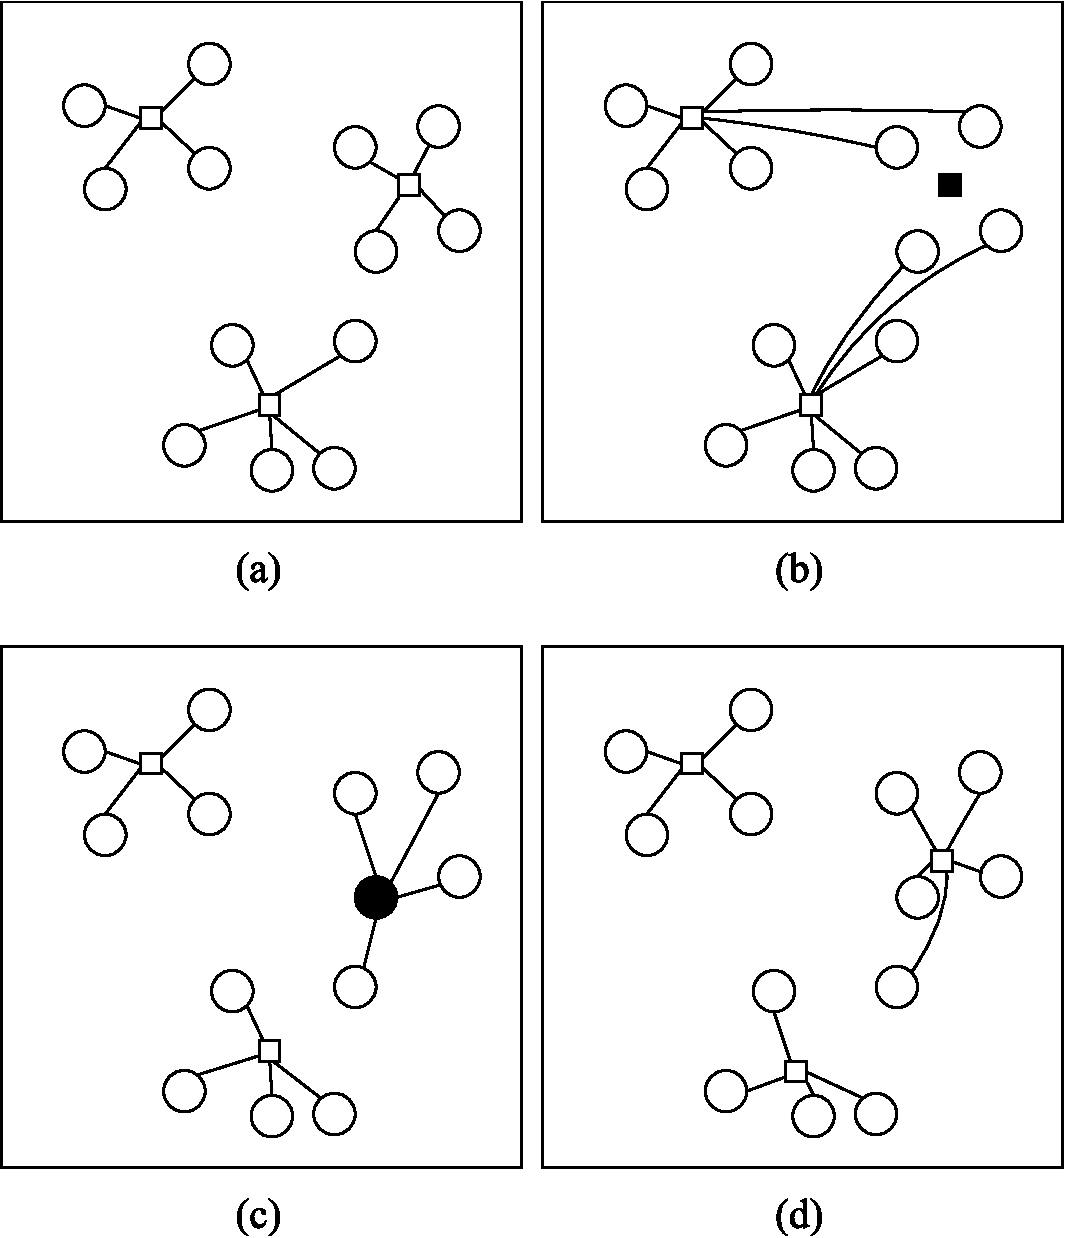
\includegraphics[width=1.0\textwidth]{img/mutation}
    \caption{Mutation based on centroid relocation: (a) selection of the centroid to be relocated; (b) re-assignments among the remaining centroids; (c) selection of the data point where the removed centroid will be placed and (d) final re-assignments and the new solution.}\label{fig:mutation}
  \end{center}
\end{figure}

\subsection{Local improvement}
\label{subsec:local-improvement}
After the generation process in crossover and mutation, $\theta'$ is enhanced by means of a local improvement procedure. The local improvement aims to find a local optimum by applying local changes to the current solution. Here, the adopted local improvement is one run of the k-means algorithm. The k-means starts with the initial solution $\theta'$ with $m$ centroids $c_1$, $c_2$, ..., $c_m$, and proceeds by alternating between two steps:

\begin{enumerate}

	\item Assignment step: Assign each data point $x_i$ to the closest cluster.
	
	\begin{equation}
	cluster(x_i) = min_j \quad d(x_i, c_j), \quad j = 1,...,m
	\end{equation}
	
	\item Update step: Calculate the new centroids $c_j$ to be the mean (average) point of the data points in the new clusters.
	
	\begin{equation}
	c_j = \frac{\sum_{x \in S_j}x}{\left | S_j \right |}, \quad j = 1,...,m
	\end{equation}
		
\end{enumerate}

Then the algorithm keeps repeating these two steps until the assignments no longer change, converging to a local optimum.

In our experiments, we use the k-means implementation of Hamerly \cite{Hamerly2010}, who proposed an acceleration that gives the same answer of the standard Lloyd's k-means \cite{Lloyd1982} but is much faster in practice. This implementation avoids distance computations by using the triangle inequality and lower bounds on distances. The time per k-means iteration of the algorithm is O($nmd$+$md^2$), where $n$ is the number of data points, $m$ is the number of clusters and $d$ is the number of data dimensions (features). However, the calculated lower bounds allow to eliminate the innermost k-means loop in around 80\% of the time, which in practise is much faster than the standard k-means.

\subsection{Treatment of incomplete solutions}
When generating new individuals, it is possible that a cluster is left empty, i.e., no data point is allocated to it. This can happen in two situations: 

\begin{itemize}
	
	\item when generating a solution in crossover or mutation, one or more centroids could not be the closest centroid to any data point;

	\item when generating a solution in the population initialization, it could happen that some numbers in the interval [ 1, ..., $m$ ] are not chosen for the assignment, as it is a random selection.
	
\end{itemize}

To work around this issue and deal only with solutions with exactly $m$ clusters, the following procedure is adopted just after the execution of crossover, mutation and population initialization if a solution with less than $m$ clusters is generated: while there is an empty cluster, select the data point farthest from its current centroid and allocate it to an empty cluster. Important: The data point selected for relocation must belong to a cluster with more than one element, otherwise the empty cluster is populated but the cluster with one data point is left empty.

\section{Population management}
\label{sec:population-management}
One of the main challenges in population-based algorithms is avoiding premature convergence of the population. The selection of parents based on elitism favours good individuals, reducing the diversity of the genetic material in the coming generations of the population. To overcome this issue, we propose a mechanism that propagates good solutions while ensuring diversity. Thus, the search procedure can be led to unexplored regions of the search space without losing promising individuals. We call \textit{Survivors selection} as this mechanism to complement the selection, crossover and local improvement operators.

%One of the main challenges in population-based algorithms is avoiding premature convergence of the population. The selection of parents based on elitism tends to favour good individuals to mate, reducing the diversity of the genetic material in the coming generations of the population. In order to overcome this issue, we propose two mechanisms that preserve the good solutions while ensuring diversity. Thus, the search procedure can be lead to unexplored regions of the search space without losing promising individuals. We call \textit{Survivors selection} and \textit{Diversification} management as these mechanisms to complement the selection, crossover and local improvement operators.

\subsection{Survivors selection}
\label{subsec:survivors}
The \textit{Survivors selection} aims to select the best individuals to propagate when the maximum population size $\Pi$ is reached. This procedure determines the $\mu$ individuals that will go on to the next generation, by discarding $\lambda$ individuals ($\lambda = \Pi - \mu$) that are either clones (identical to other solution) or bad regarding the fitness, according to algorithm \ref{survivors}.

This characteristic of eliminating clones and poor solutions reveals two aspects of the \textit{Survivors selection} mechanism. The first one is that population diversity is maintained, as we favour the removal of clones first. The second is related to elitism, as the individuals with good fitness are preserved. %Other aspects related to diversity can be observed in mutation and diversification operators.

\begin{algorithm}[H]
\caption{Survivors selection}
\label{survivors}
\begin{algorithmic}[1]
\FOR{$i = 1 ... \lambda$}
\STATE $X \leftarrow $ all individuals having a clone
\IF{$X \neq \emptyset$}
\STATE Remove $p \in X$ with minimum fitness
\ELSE
\STATE Remove $p$ in the population with minimum fitness
\ENDIF
\ENDFOR
\end{algorithmic}
\end{algorithm}

%\subsection{Diversification management}
%\label{subsec:diversification}
%The \textit{Diversification} mechanism aims to ensure the genetic diversity in a population. It is actually a complementary procedure to diversify the population of solutions, once the mutation carries the most important role regarding this matter. \textit{Diversification} is called after the survivors selection whenever $I_D$ iterations happen without improving the best solution. It is performed by creating $\beta$ new individuals as in the initialization phase, i.e., individuals are randomly generated and then submitted to local improvement. As this process introduces a significant amount of new genetic material, it allows the exploration of unvisited regions of the search space.

\section{Computational complexity}
\label{sec:complexity-algo}
As stated in previous sections, after the initialization of the population, the proposed meta-heuristic operates in an external loop that calls some internal operators. Among these operators, the main bottleneck is the local improvement phase, where the K-means is performed to improve the newly mutated solution. As the computational complexity of K-means is $O(nmd + md^2)$ \cite{Hamerly2010}, the overall complexity of the proposed algorithm is $O(I_{max} (nmd + md^2))$, as the local improvement is applied after the mutation in each iteration (the maximum number of iterations in the external loop is $I_{max}$). Thus, although the proposed meta-heuristic is of the same asymptotic complexity of k-means, it is in practice slower than K-means due to the constant $I_{max}$ set in the external loop and to other internal operators, like crossover, mutation, survivors selection and diversification. In the following, the computational complexity of each internal operator:

%- initial population: $O(100 * (nmd + md^2))$

%- main GA loop: $O(I_{max})$ (constant)

\begin{itemize}

	\item Selection: $O(w)$ ($w$ constant)

	\item Crossover: $O(nmd + m^{3})$

	\item Mutation: $O(nmd)$

	\item Local improvement (k-means): $O(nmd + md^2)$

\end{itemize}
%$^{*}$ $O(nmd)$ because $n$ is typically much greater than $m$, but for $n < m$ the crossover complexity becomes $O(m^{3})$ due to the Hungarian algorithm for finding the matching between centroids.

%In addition to the above internal operators, the mechanisms for population management are also performed in the general loop. However, unlike the other operators, \textit{Survivors selection} and \textit{Diversification} are not performed on each iteration, but only when some criteria are reached. \textit{Survivors selection} is performed whenever the population reaches $\Pi$ individuals; and \textit{Diversification} is called after the \textit{Survivors selection} if $I_D$ iterations happen without improving the best solution. Therefore, their contribution to the computational time of the algorithm is small in practice. Their complexities are:

In addition to the above internal operators, a mechanism to select the best individuals for propagation is also performed in the general loop. However, unlike the other operators, the \textit{Survivors selection} is not performed on each iteration, but only when the population reaches $\Pi$ individuals. Therefore, its contribution to the computational time of the algorithm is small in practice. Its complexity is:

\begin{itemize}

	\item Survivors selection: $O(n\Pi)$

	%\item Diversification: $O(\beta (nmd + md^2))$ ($\beta$ constant)

\end{itemize}
  \chapter{Computational Experiments and Analysis}
\label{chap:experiments}
In this chapter, we discuss the computational experiments and the analysis that emerge from them. From now on, all results regarding the proposed algorithm will be identified as HGKM (for Hybrid Genetic K-Means). The results are presented in terms of objective function value and time, and are compared to current state-of-the-art results in the MSSC literature.

The experiments were conducted on an Intel Core i5 2.6 GHz processor machine with 8 GB of RAM memory. The source codes were written in C++, using the UNIX g++ compiler on a Linux Ubuntu 14.04 LTS 64-bit operating system.

Three different analysis are presented in this chapter. The first one analyses the general performance of the proposed algorithm in terms of objective function value and computational time, where we compare our results with the current literature. The second one analyses the impact of instances characteristics, where the objective is to verify if the proposed algorithm is affected by the number of clusters and the size of instances. Finally, we analyse the contribution of crossover and mutation components in the performance of the method.

In the coming result tables, the following notation is used:

\begin{itemize}
	\item $n$ is the size of the instance (number of data points);
	
	\item $m$ is the number of clusters;

	\item $d$ is the number of features;
	
	\item $f_{best}$ is the best known value for the MSSC objective found so far;

	\item $E$ is the error from the best known solution, calculated as:

		\begin{center}
		\large
			$E = \frac{f - f_{best}}{f_{best}} \times 100$
		\end{center}
		
	where $f$ is the value of the MSSC objective found by an algorithm. For HGKM, $E_{med}$ and $E_{avg}$ report the error from the median and average values, respectively;
	
	\item $t$ is the CPU time in seconds;
	
	%\item Bold values are used when HGKM found the new best solution

\end{itemize}

\section{Instances}
\label{sec:instances}
The selection of instances was done in order to cover different types of real data, considering both the instance size and the number of features as important indicators to describe the nature of data. Table \ref{instances} summarizes the characteristics of the adopted instances, which correspond to 24 important benchmarks in recent clustering literature, as reported in \cite{Ordin2014} and \cite{Bagirov2016}. For all considered instances, every feature value is a real or integer number and there is no missing values. The number of data points (instances size) ranges from 59 (smallest) to 434,874 (largest); and the number of features ranges from 2 (smallest) to 128 (largest).

In order to elucidate the coming analysis, we propose the discrimination of these instances according to their sizes, that from now on will by identified as Group A1, Group A2, Group B and Group C of instances.

Groups A1 and A2 correspond to small instances reported in the work of \cite{Ordin2014}. The difference between them is that A1 is composed by really small instances with up to 150 data points, where instances in A2 have some hundreds of data points. This distinction is useful to choose a reasonable number of clusters to be tested in each group. For instances A1, tests are performed considering up to 10 clusters, whereas in A2 we can extend a bit the number of clusters. Group B of instances correspond to medium/large instances reported also by \cite{Ordin2014}, comprising data where the number of points ranges from 1,060 to 20,000. Group C of instances are the same reported in \cite{Bagirov2016}, where instance sizes ranges from 13,910 to 434,874 data points. This last group is especially relevant as it consider large real world instances, which allows a deeper analysis in the scaling of algorithms.

% -*- coding: utf-8; -*-
\begin{table}[]
\centering
\begin{tabular}{@{}llc@{}}
\toprule
Instance                        & Number of data points & Number of features \\ \midrule
German towns                    & 59                    & 2                  \\
Bavaria postal 1                & 89                    & 3                  \\
Bavaria postal 2                & 89                    & 4                  \\
Fisher’s Iris Plant             & 150                   & 4                  \\
Heart Disease                   & 297                   & 13                 \\
Liver Disorders                 & 345                   & 6                  \\
Ionosphere                      & 351                   & 34                 \\
Congressional Voting Records    & 435                   & 16                 \\
Breast Cancer                   & 683                   & 9                  \\
Pima Indians Diabetes           & 768                   & 8                  \\
TSPLIB1060                      & 1060                  & 2                  \\
Image Segmentation              & 2310                  & 19                 \\
TSPLIB3038                      & 3038                  & 2                  \\
Page Blocks                     & 5473                  & 10                 \\
Pendigit                        & 10992                 & 16                 \\
Gas sensor                      & 13910                 & 128                \\
EEG eye state                   & 14980                 & 14                 \\
D15112                          & 15112                 & 2                  \\
Letters                         & 20000                 & 16                 \\
KEGG metabolic relation network & 53413                 & 20                 \\
Shuttle control                 & 58000                 & 9                  \\
Pla85900                        & 85900                 & 2                  \\
Skin Segmentation               & 245057                & 3                  \\
3D road network                 & 434874                & 3                  \\ \bottomrule
\end{tabular}
\caption{Instances description}
\label{instances}
\end{table}

\section{Parameters calibration}
\label{sec:calibration}
As in most meta-heuristics, the values chosen for parameters directly affect the results. In this work, we consider five main parameters: $w$ (the tournament size for selection), $\mu$ (the population size), $\Pi$ (the maximum size of population), $I_{max}$ (the maximum number of iterations) and $I_S$ (the number of iterations without improvement that causes the algorithm stop). For the parameters related to the management of individuals in the population ($w$, $\mu$ and $\Pi$) we performed a calibration to choose the best configuration for the experiments. For the parameters related to the number of iterations the algorithm takes ($I_{max}$ and $I_S$), we directly set their values to 4000 and 2500, respectively. These values were set in order to obtain results in a time comparable to previous authors.

In preliminary experiments, we started with the following configuration for the free variables, as they produced good and stable results after an initial and manually exploration: $w$ = 3, $\mu$ = 80 and $\Pi$ = 300. From this baseline, we expanded the range of these values by an one-factor-at-a-time (OFAT) approach. Table \ref{calibration} presents the ranges of tested values for each parameter and the final values achieved after increasing/decreasing each parameter value at a time.

% -*- coding: utf-8; -*-
\begin{table}[H]
\centering
\begin{tabular}{@{}lllc@{}}
\toprule
\multicolumn{2}{l}{Parameter}           & Range of values             & Final value \\ \midrule
$w$     & Tournament size for selection & \{2, 3, 4\}                 & 3           \\
$\mu$   & Population size               & \{60, 70, 80, 90, 100\}     & 80          \\
$\Pi$   & Maximum size of population    & \{200, 250, 300, 350, 400\} & 200         \\ \bottomrule
\end{tabular}
\caption{Parameters calibration}
\label{calibration}
\end{table}

We considered a subset of five instances for calibration, that were chosen based on their sizes and number of features (Liver disorders, Ionosphere, Breast cancer, Pima Indians diabetes and TSPLIB1060). Small instances were not considered because in almost all of them the different configurations for calibration achieved the best known result (possibly the global optimal), so they are not so informative. As we consider 3 parameters independently, the combination of parameters resulted in 11 possible configurations, as shown in table \ref{calibration-results}. For this reason, large instances were not considered.
%It would take too much time just to calibrate the algorithm, as we run 10 times each experiment.
We chose medium-sized instances and tested 4 different number of clusters (20, 30, 40, 50) for each instance. After measuring the offset between the average error and the execution time for each configuration, we took the best one among the 11 options.

In table \ref{calibration-results}, the first three columns report the values of parameters $w$, $\mu$ and $\Pi$, whereas the remaining columns report, in turn, the errors from the best, worst, median and average solution, and finally the average time taken to run the considered instances for calibration.

\begin{table}[!h]
\centering
\begin{tabular}{@{}cccccccc@{}}
\toprule
$w$ & $\mu$ & $\Pi$ & $E_{bst}$  & $E_{wst}$ & $E_{med}$ & $E_{avg}$ & Total Time \\ \midrule
3   & 80    & 300   & -4.70      & 0.28      & -0.88     & -1.24     & 940.63     \\
2   & 80    & 300   & -4.83      & 0.27      & -0.81     & -1.25     & 1002.89    \\
4   & 80    & 300   & -4.53      & 0.19      & -0.90     & -1.22     & 854.62     \\
3   & 60    & 300   & -4.86      & 0.34      & -0.93     & -1.21     & 885.68     \\
3   & 70    & 300   & -4.85      & 0.25      & -0.95     & -1.23     & 917.79     \\
3   & 90    & 300   & -4.77      & 0.61      & -0.81     & -1.23     & 957.70     \\
3   & 100   & 300   & -4.80      & 0.34      & -0.73     & -1.23     & 978.47     \\
3   & 80    & 200   & -4.80      & 0.19      & -0.88     & -1.23     & 875.21     \\
3   & 80    & 250   & -4.87      & 0.40      & -0.78     & -1.24     & 1001.25    \\
3   & 80    & 350   & -4.85      & 0.41      & -0.79     & -1.25     & 1017.34    \\
3   & 80    & 400   & -4.91      & 0.32      & -0.76     & -1.26     & 999.21     \\
%2   & 80    & 300   & -4.96      & 0.55      & -0.76     & -1.21     & 960.46     \\
%2   & 60    & 230   & -4.76      & 0.19      & -0.79     & -1.22     & 840.16     \\
%2   & 80    & 300   & -4.92      & 0.70      & -0.72     & -1.18     & 805.58     \\
%2   & 60    & 230   & -4.75      & 0.89      & -0.74     & -1.18     & 804.05     \\
\bottomrule
\end{tabular}
\caption{Results of calibration}
\label{calibration-results}
\end{table}

\section{Experimental results}
\label{sec:results}

\subsection{General performance and computational time}
\label{sec:performance}
The results of numerical experiments regarding solution performance and computational time for groups A1, A2, B and C of instances are presented in tables \ref{results-all-A1}, \ref{results-all-A2}, \ref{results-all-B} and \ref{results-all-C}, respectively. Due to the stochastic nature of the proposed meta-heuristic, the results of HGKM correspond to the average of 10 runs, where a run is the execution of an instance with a specific $m$. 

For comparison purposes, we analyse the results considering the best known solutions found so far and the results of global K-means (GKM) \cite{Likas2003}, the modified global K-means (MGKM) \cite{Bagirov2008}, the multi-start modified global K-means (MS-MGKM) \cite{Ordin2014} and the difference of convex clustering (DCC) \cite{Bagirov2016} algorithms, which are recent works in MSSC literature, corresponding in many cases to the state-of-the-art for this problem.

% HGKM performance analysis
Tables \ref{results-all-A1} and \ref{results-all-A2} presents the results for instances of group A1 and A2. As we can observe, HGKM finds the new best solution or achieves the current best one in all instances for most of $m$ values. In some cases, as in Ionosphere instance, HGKM results reach more than 4\% of the error, being a significant improvement. On the other hand, the proposed algorithm requires more computational efforts than MS-MGKM, MGKM and GKM algorithms for most of these small instances -- in many cases the computational time of HGKM is similar to MS-MGKM. It is also important to note that in some instances like Bavaria postal 2, Liver disorders, Ionosphere and Pima Indians diabetes, the gap of HGKM results to the best known solutions increases for large $m$, which means that for harder clustering tasks HGKM produces significantly better solutions than the compared algorithms.

Table \ref{results-all-B} presents the results for instances of group B. As in results for small instances, HGKM finds the new best solution or achieves the current best one in all instances for most of $m$ values, being better than algorithms MS-MGKM, MGKM and GKM in terms of solution quality. Regarding computational time, HGKM is faster than MS-MGKM and GKM in TSPLIB3038, faster than MS-MGKM in TSPLIB1060 and has nearly the same time of MS-MGKM and MGKM in Pendigit. For Image segmentation and Page Block -- the latter, only for large $m$ -- HGKM requires more computational effort.

Table \ref{results-all-C} presents the results for instances of group C -- the group with the largest instances. As in the previous results, HGKM finds the new best solution or achieves the current best one in all instances for most of $m$ values. Regarding computational time, HGKM is faster than MS-MGKM, DCCClust, MS-DCA and GKM for almost all instances, except for EEG eye state and D15112.

{\footnotesize
\centering
\begin{longtable}{@{}llccccccccc@{}}
m  & $f_{best}$ & \multicolumn{2}{c}{MS-MGKM} & \multicolumn{2}{c}{MGKM} & \multicolumn{2}{c}{GKM} & \multicolumn{3}{c}{HGKM}      \\ \midrule
   &            & $E$          & $t$          & $E$         & $t$        & $E$         & $t$       & $E_{med}$ & $E_{avg}$ & $t$   \\
\multicolumn{11}{l}{German towns}                                                                                                  \\
2  & 121430     & 0.00         & 0.00         & 0.00        & 0.00       & 0.00        & 0.00      & 0.00      & 0.00      & 0.07  \\
3  & 77009      & 0.00         & 0.02         & 1.45        & 0.00       & 1.45        & 0.00      & 0.00      & 0.00      & 0.07  \\
4  & 49601      & 0.24         & 0.02         & 0.72        & 0.00       & 0.72        & 0.00      & 0.00      & 0.00      & 0.08  \\
5  & 38716      & 0.00         & 0.02         & 0.00        & 0.00       & 0.00        & 0.00      & 0.00      & 0.00      & 0.08  \\
6  & 30536      & 0.00         & 0.02         & 0.27        & 0.00       & 0.00        & 0.00      & 0.00      & 0.00      & 0.08  \\
7  & 24433      & 0.08         & 0.02         & 0.00        & 0.00       & 0.09        & 0.00      & 0.00      & 0.00      & 0.09  \\
8  & 21631      & 0.00         & 0.02         & 0.54        & 0.00       & 0.64        & 0.00      & -0.68     & -0.68     & 0.10  \\
9  & 18550      & 2.13         & 0.02         & 4.46        & 0.00       & 2.13        & 0.00      & 0.00      & 0.00      & 0.10  \\
10 & 16307      & 1.81         & 0.02         & 1.52        & 0.00       & 1.81        & 0.00      & 0.01      & 0.01      & 0.11  \\
\multicolumn{11}{l}{Bavaria postals 1}                                                                                             \\
2  & 6.0255E+11 & 0.00         & 0.02         & 0.00        & 0.00       & 0.00        & 0.00      & 0.00      & 0.00      & 0.11  \\
3  & 2.9451E+11 & 0.00         & 0.02         & 0.01        & 0.00       & 0.01        & 0.00      & 0.00      & 0.00      & 0.18  \\
4  & 1.0447E+11 & 0.05         & 0.02         & 0.05        & 0.00       & 0.05        & 0.00      & 0.00      & 0.00      & 0.20  \\
5  & 5.9762E+10 & 0.06         & 0.03         & 0.54        & 0.02       & 0.54        & 0.02      & 0.00      & 0.00      & 0.21  \\
6  & 3.5909E+10 & 0.07         & 0.03         & 1.44        & 0.02       & 1.44        & 0.02      & 0.00      & 0.00      & 0.28  \\
7  & 2.1983E+10 & 0.01         & 0.05         & 3.17        & 0.02       & 3.17        & 0.02      & 0.00      & 0.00      & 0.28  \\
8  & 1.3385E+10 & 0.25         & 0.06         & 1.71        & 0.02       & 1.71        & 0.02      & 0.00      & 0.00      & 0.31  \\
9  & 8.4237E+9  & 0.28         & 0.08         & 2.85        & 0.02       & 2.85        & 0.02      & 0.00      & 0.00      & 0.38  \\
10 & 6.4465E+9  & 0.07         & 0.09         & 3.55        & 0.02       & 3.55        & 0.02      & 0.00      & 0.00      & 0.44  \\
\multicolumn{11}{l}{Bavaria postals 2}                                                                                             \\
2  & 4.8631E+10 & 0.00         & 0.00         & 0.00        & 0.00       & 7.75        & 0.00      & 0.00      & 0.00      & 0.07  \\
3  & 1.7399E+10 & 0.00         & 0.00         & 0.00        & 0.00       & 0.00        & 0.00      & 0.00      & 0.00      & 0.08  \\
4  & 7.5591E+9  & 0.00         & 0.00         & 0.00        & 0.00       & 0.00        & 0.00      & 0.00      & 0.00      & 0.09  \\
5  & 5.3429E+9  & 0.00         & 0.00         & 0.00        & 0.00       & 0.00        & 0.00      & 0.00      & 0.00      & 0.10  \\
6  & 3.1876E+9  & 0.00         & 0.00         & 0.00        & 0.00       & 0.00        & 0.00      & 0.00      & 0.00      & 0.11  \\
7  & 2.2159E+9  & 0.61         & 0.00         & 1.50        & 0.02       & 1.50        & 0.00      & -0.04     & -0.04     & 0.13  \\
8  & 1.7045E+9  & 0.00         & 0.02         & 0.00        & 0.02       & 0.00        & 0.00      & 0.00      & 0.00      & 0.13  \\
9  & 1.4030E+9  & 0.00         & 0.02         & 0.00        & 0.02       & 0.00        & 0.00      & -0.14     & -0.14     & 0.14  \\
10 & 1.1841E+9  & 0.00         & 0.02         & 0.00        & 0.02       & 0.00        & 0.00      & -0.26     & -0.26     & 0.15  \\
\multicolumn{11}{l}{Fisher Iris}                                                                                                   \\
2  & 152.348    & 0.00         & 0.00         & 7.32        & 0.00       & 7.32        & 0.00      & 0.00      & 0.00      & 0.08  \\
3  & 78.851     & 0.00         & 0.00         & 0.00        & 0.00       & 0.00        & 0.00      & 0.00      & 0.00      & 0.09  \\
4  & 57.228     & 0.00         & 0.00         & 0.00        & 0.00       & 0.00        & 0.00      & 0.00      & 0.00      & 0.10  \\
5  & 46.446     & 0.00         & 0.00         & 1.86        & 0.00       & 1.86        & 0.00      & 0.00      & 0.00      & 0.12  \\
6  & 39.040     & 0.00         & 0.00         & 1.21        & 0.02       & 1.21        & 0.00      & 0.00      & 0.00      & 0.12  \\
7  & 34.298     & 0.00         & 0.00         & 0.51        & 0.02       & 0.51        & 0.00      & 0.00      & 0.00      & 0.14  \\
8  & 29.989     & 0.18         & 0.02         & 0.73        & 0.02       & 0.73        & 0.00      & 0.00      & 0.00      & 0.16  \\
9  & 27.786     & 1.07         & 0.02         & 0.00        & 0.02       & 0.00        & 0.00      & 0.00      & 0.00      & 0.18  \\
10 & 25.834     & 0.00         & 0.02         & 0.73        & 0.02       & 0.73        & 0.00      & 0.00      & 0.00      & 0.20  \\ \bottomrule
\caption{Objective value and time obtained by algorithms in instances of group A1.}\\
\label{results-all-A1}\\
\end{longtable}}


{\footnotesize
\centering
\begin{longtable}{@{}llccccccccc@{}}
\hline
\multicolumn{1}{l|}{m}  & \multicolumn{1}{l|}{$f_{best}$} & \multicolumn{2}{c|}{MS-MGKM}      & \multicolumn{2}{c|}{MGKM}         & \multicolumn{2}{c|}{GKM}          & \multicolumn{3}{c}{HGKM}      \\ \hline
                        & \multicolumn{1}{l|}{}           & $E$  & \multicolumn{1}{c|}{$t$}   & $E$   & \multicolumn{1}{c|}{$t$}  & $E$   & \multicolumn{1}{c|}{$t$}  & E$_{med}$ & E$_{avg}$ & $t$   \\ \hline
\multicolumn{11}{l}{Heart disease}                                                                                                                                                                    \\ \hline
\multicolumn{1}{l|}{2}  & \multicolumn{1}{l|}{598900}     & 0.00 & \multicolumn{1}{c|}{0.03}  & 93.96 & \multicolumn{1}{c|}{0.00} & 93.96 & \multicolumn{1}{c|}{0.00} & 0.00      & 0.00      & 0.48  \\
\multicolumn{1}{l|}{5}  & \multicolumn{1}{l|}{327970}     & 0.01 & \multicolumn{1}{c|}{0.13}  & 0.08  & \multicolumn{1}{c|}{0.03} & 0.08  & \multicolumn{1}{c|}{0.03} & 0.00      & 0.00      & 1.01  \\
\multicolumn{1}{l|}{10} & \multicolumn{1}{l|}{200650}     & 0.00 & \multicolumn{1}{c|}{0.63}  & 6.96  & \multicolumn{1}{c|}{0.08} & 6.93  & \multicolumn{1}{c|}{0.05} & -0.06     & -0.06     & 1.91  \\
\multicolumn{1}{l|}{15} & \multicolumn{1}{l|}{147650}     & 0.00 & \multicolumn{1}{c|}{1.20}  & 0.06  & \multicolumn{1}{c|}{0.13} & 1.69  & \multicolumn{1}{c|}{0.08} & -0.55     & -0.55     & 2.45  \\
\multicolumn{1}{l|}{20} & \multicolumn{1}{l|}{117780}     & 0.00 & \multicolumn{1}{c|}{1.77}  & 0.77  & \multicolumn{1}{c|}{0.19} & 1.07  & \multicolumn{1}{c|}{0.11} & -0.86     & -0.86     & 3.15  \\
\multicolumn{1}{l|}{25} & \multicolumn{1}{l|}{99292}      & 0.00 & \multicolumn{1}{c|}{2.61}  & 1.74  & \multicolumn{1}{c|}{0.28} & 1.98  & \multicolumn{1}{c|}{0.13} & -0.82     & -0.78     & 3.66  \\
\multicolumn{1}{l|}{30} & \multicolumn{1}{l|}{86216}      & 0.00 & \multicolumn{1}{c|}{3.28}  & 1.36  & \multicolumn{1}{c|}{0.39} & 1.57  & \multicolumn{1}{c|}{0.16} & -0.54     & -0.48     & 4.38  \\
\multicolumn{1}{l|}{40} & \multicolumn{1}{l|}{67701}      & 0.00 & \multicolumn{1}{c|}{4.67}  & 1.05  & \multicolumn{1}{c|}{0.66} & 4.68  & \multicolumn{1}{c|}{0.23} & -1.69     & -1.44     & 5.15  \\
\multicolumn{1}{l|}{50} & \multicolumn{1}{l|}{54878}      & 0.00 & \multicolumn{1}{c|}{6.06}  & 3.33  & \multicolumn{1}{c|}{0.97} & 9.01  & \multicolumn{1}{c|}{0.28} & -1.06     & -1.01     & 6.18  \\ \hline
\multicolumn{11}{l}{Liver disorders}                                                                                                                                                                  \\ \hline
\multicolumn{1}{l|}{2}  & \multicolumn{1}{l|}{423980}     & 0.00 & \multicolumn{1}{c|}{0.08}  & 0.00  & \multicolumn{1}{c|}{0.05} & 0.00  & \multicolumn{1}{c|}{0.03} & 0.00      & 0.00      & 0.27  \\
\multicolumn{1}{l|}{5}  & \multicolumn{1}{l|}{218260}     & 0.06 & \multicolumn{1}{c|}{0.39}  & 0.18  & \multicolumn{1}{c|}{0.13} & 0.07  & \multicolumn{1}{c|}{0.05} & 0.00      & 0.00      & 0.65  \\
\multicolumn{1}{l|}{10} & \multicolumn{1}{l|}{119400}     & 0.00 & \multicolumn{1}{c|}{0.81}  & 0.64  & \multicolumn{1}{c|}{0.27} & 2.38  & \multicolumn{1}{c|}{0.08} & 6.71      & 6.71      & 1.46  \\
\multicolumn{1}{l|}{15} & \multicolumn{1}{l|}{97405}      & 0.00 & \multicolumn{1}{c|}{1.39}  & 0.81  & \multicolumn{1}{c|}{0.42} & 5.16  & \multicolumn{1}{c|}{0.11} & -0.67     & -0.67     & 1.84  \\
\multicolumn{1}{l|}{20} & \multicolumn{1}{l|}{81192}      & 0.00 & \multicolumn{1}{c|}{1.86}  & 1.52  & \multicolumn{1}{c|}{0.77} & 7.33  & \multicolumn{1}{c|}{0.13} & -1.41     & -1.40     & 2.72  \\
\multicolumn{1}{l|}{25} & \multicolumn{1}{l|}{69212}      & 0.00 & \multicolumn{1}{c|}{2.42}  & 0.68  & \multicolumn{1}{c|}{1.39} & 7.49  & \multicolumn{1}{c|}{0.16} & -1.90     & -1.74     & 3.30  \\
\multicolumn{1}{l|}{30} & \multicolumn{1}{l|}{60325}      & 0.00 & \multicolumn{1}{c|}{3.09}  & 0.37  & \multicolumn{1}{c|}{2.20} & 7.77  & \multicolumn{1}{c|}{0.20} & -2.25     & -2.11     & 3.66  \\
\multicolumn{1}{l|}{40} & \multicolumn{1}{l|}{47336}      & 0.87 & \multicolumn{1}{c|}{4.98}  & 0.00  & \multicolumn{1}{c|}{4.77} & 7.82  & \multicolumn{1}{c|}{0.30} & -1.13     & -1.04     & 4.55  \\
\multicolumn{1}{l|}{50} & \multicolumn{1}{l|}{38305}      & 0.28 & \multicolumn{1}{c|}{6.89}  & 0.00  & \multicolumn{1}{c|}{8.39} & 6.63  & \multicolumn{1}{c|}{0.38} & -1.55     & -1.50     & 5.20  \\ \hline
\multicolumn{11}{l}{Ionosphere}                                                                                                                                                                       \\ \hline
\multicolumn{1}{l|}{2}  & \multicolumn{1}{l|}{2419.4}     & 0.00 & \multicolumn{1}{c|}{0.09}  & 0.00  & \multicolumn{1}{c|}{0.06} & 0.00  & \multicolumn{1}{c|}{0.05} & 0.00      & 0.00      & 1.12  \\
\multicolumn{1}{l|}{5}  & \multicolumn{1}{l|}{1891.5}     & 0.00 & \multicolumn{1}{c|}{0.58}  & 1.86  & \multicolumn{1}{c|}{0.17} & 2.28  & \multicolumn{1}{c|}{0.09} & -0.09     & -0.09     & 2.76  \\
\multicolumn{1}{l|}{10} & \multicolumn{1}{l|}{1559.4}     & 0.00 & \multicolumn{1}{c|}{1.06}  & 0.13  & \multicolumn{1}{c|}{0.33} & 0.11  & \multicolumn{1}{c|}{0.17} & -0.60     & -0.58     & 3.97  \\
\multicolumn{1}{l|}{15} & \multicolumn{1}{l|}{1390.1}     & 0.00 & \multicolumn{1}{c|}{1.72}  & 0.92  & \multicolumn{1}{c|}{0.48} & 0.88  & \multicolumn{1}{c|}{0.23} & -2.18     & -2.16     & 5.54  \\
\multicolumn{1}{l|}{20} & \multicolumn{1}{l|}{1252.4}     & 0.00 & \multicolumn{1}{c|}{2.48}  & 1.17  & \multicolumn{1}{c|}{0.66} & 2.99  & \multicolumn{1}{c|}{0.31} & -2.75     & -2.69     & 7.04  \\
\multicolumn{1}{l|}{25} & \multicolumn{1}{l|}{1140.8}     & 0.00 & \multicolumn{1}{c|}{3.38}  & 0.31  & \multicolumn{1}{c|}{0.83} & 4.45  & \multicolumn{1}{c|}{0.38} & -3.34     & -3.28     & 8.38  \\
\multicolumn{1}{l|}{30} & \multicolumn{1}{l|}{1043.0}     & 0.00 & \multicolumn{1}{c|}{4.27}  & 1.28  & \multicolumn{1}{c|}{0.98} & 4.75  & \multicolumn{1}{c|}{0.45} & -4.44     & -4.39     & 9.88  \\
\multicolumn{1}{l|}{40} & \multicolumn{1}{l|}{856.6}      & 0.00 & \multicolumn{1}{c|}{5.59}  & 2.36  & \multicolumn{1}{c|}{1.39} & 6.14  & \multicolumn{1}{c|}{0.61} & -3.58     & -3.46     & 13.11 \\
\multicolumn{1}{l|}{50} & \multicolumn{1}{l|}{702.6}      & 0.00 & \multicolumn{1}{c|}{6.75}  & 3.68  & \multicolumn{1}{c|}{1.83} & 8.05  & \multicolumn{1}{c|}{0.77} & -3.72     & -3.51     & 16.79 \\ \hline
\multicolumn{11}{l}{Congressional vote}                                                                                                                                                               \\ \hline
\multicolumn{1}{l|}{2}  & \multicolumn{1}{l|}{1640.9}     & 0.00 & \multicolumn{1}{c|}{0.13}  & 0.00  & \multicolumn{1}{c|}{0.09} & 0.00  & \multicolumn{1}{c|}{0.06} & 0.00      & 0.00      & 0.72  \\
\multicolumn{1}{l|}{5}  & \multicolumn{1}{l|}{1335.8}     & 0.03 & \multicolumn{1}{c|}{0.38}  & 0.14  & \multicolumn{1}{c|}{0.22} & 0.14  & \multicolumn{1}{c|}{0.13} & 0.00      & 0.00      & 2.28  \\
\multicolumn{1}{l|}{10} & \multicolumn{1}{l|}{1123.3}     & 0.00 & \multicolumn{1}{c|}{0.91}  & 1.86  & \multicolumn{1}{c|}{0.41} & 1.86  & \multicolumn{1}{c|}{0.20} & -0.32     & -0.31     & 4.28  \\
\multicolumn{1}{l|}{15} & \multicolumn{1}{l|}{992.07}     & 0.00 & \multicolumn{1}{c|}{1.73}  & 0.36  & \multicolumn{1}{c|}{0.59} & 0.33  & \multicolumn{1}{c|}{0.30} & -0.84     & -0.75     & 5.31  \\
\multicolumn{1}{l|}{20} & \multicolumn{1}{l|}{906.47}     & 0.00 & \multicolumn{1}{c|}{2.98}  & 0.71  & \multicolumn{1}{c|}{0.80} & 0.34  & \multicolumn{1}{c|}{0.39} & -1.51     & -1.47     & 5.62  \\
\multicolumn{1}{l|}{25} & \multicolumn{1}{l|}{839.75}     & 0.00 & \multicolumn{1}{c|}{4.97}  & 0.92  & \multicolumn{1}{c|}{0.98} & 0.37  & \multicolumn{1}{c|}{0.52} & -2.28     & -2.22     & 6.57  \\
\multicolumn{1}{l|}{30} & \multicolumn{1}{l|}{776.77}     & 0.00 & \multicolumn{1}{c|}{8.75}  & 0.98  & \multicolumn{1}{c|}{1.22} & 2.83  & \multicolumn{1}{c|}{0.59} & -1.45     & -1.48     & 6.93  \\
\multicolumn{1}{l|}{40} & \multicolumn{1}{l|}{689.35}     & 0.00 & \multicolumn{1}{c|}{12.61} & 1.81  & \multicolumn{1}{c|}{1.70} & 1.28  & \multicolumn{1}{c|}{0.83} & -2.88     & -2.84     & 8.48  \\
\multicolumn{1}{l|}{50} & \multicolumn{1}{l|}{617.5}      & 0.00 & \multicolumn{1}{c|}{15.17} & 1.73  & \multicolumn{1}{c|}{2.28} & 1.98  & \multicolumn{1}{c|}{1.06} & -3.39     & -3.32     & 10.18 \\ \hline
\multicolumn{11}{l}{Breast cancer}                                                                                                                                                                    \\ \hline
\multicolumn{1}{l|}{2}  & \multicolumn{1}{l|}{19323}      & 0.00 & \multicolumn{1}{c|}{0.05}  & 0.00  & \multicolumn{1}{c|}{0.02} & 0.00  & \multicolumn{1}{c|}{0.02} & 0.00      & 0.00      & 0.58  \\
\multicolumn{1}{l|}{5}  & \multicolumn{1}{l|}{13705}      & 0.00 & \multicolumn{1}{c|}{0.27}  & 0.52  & \multicolumn{1}{c|}{0.05} & 0.52  & \multicolumn{1}{c|}{0.02} & 0.00      & 0.00      & 1.64  \\
\multicolumn{1}{l|}{10} & \multicolumn{1}{l|}{10205}      & 0.00 & \multicolumn{1}{c|}{0.94}  & 2.70  & \multicolumn{1}{c|}{0.09} & 0.75  & \multicolumn{1}{c|}{0.03} & -0.14     & -0.14     & 3.02  \\
\multicolumn{1}{l|}{15} & \multicolumn{1}{l|}{8704.7}     & 0.00 & \multicolumn{1}{c|}{1.47}  & 0.72  & \multicolumn{1}{c|}{0.17} & 0.04  & \multicolumn{1}{c|}{0.06} & -0.80     & -0.74     & 4.74  \\
\multicolumn{1}{l|}{20} & \multicolumn{1}{l|}{7695.2}     & 0.39 & \multicolumn{1}{c|}{1.94}  & 1.34  & \multicolumn{1}{c|}{0.23} & 0.00  & \multicolumn{1}{c|}{0.09} & -1.19     & -1.13     & 6.79  \\
\multicolumn{1}{l|}{25} & \multicolumn{1}{l|}{6946.4}     & 0.00 & \multicolumn{1}{c|}{2.47}  & 2.86  & \multicolumn{1}{c|}{0.33} & 3.35  & \multicolumn{1}{c|}{0.11} & -0.88     & -0.81     & 7.55  \\
\multicolumn{1}{l|}{30} & \multicolumn{1}{l|}{6360.3}     & 0.00 & \multicolumn{1}{c|}{3.08}  & 3.31  & \multicolumn{1}{c|}{0.44} & 2.99  & \multicolumn{1}{c|}{0.14} & -0.40     & -0.32     & 8.79  \\
\multicolumn{1}{l|}{40} & \multicolumn{1}{l|}{5487.8}     & 0.00 & \multicolumn{1}{c|}{4.05}  & 1.39  & \multicolumn{1}{c|}{0.69} & 3.13  & \multicolumn{1}{c|}{0.20} & -0.62     & -0.64     & 9.87  \\
\multicolumn{1}{l|}{50} & \multicolumn{1}{l|}{4812.3}     & 0.00 & \multicolumn{1}{c|}{5.20}  & 1.85  & \multicolumn{1}{c|}{1.03} & 3.95  & \multicolumn{1}{c|}{0.27} & -1.21     & -1.21     & 11.60 \\ \hline
\multicolumn{11}{l}{Pima Indians diabetes}                                                                                                                                                            \\ \hline
\multicolumn{1}{l|}{2}  & \multicolumn{1}{l|}{5.1424E+6}  & 0.00 & \multicolumn{1}{c|}{0.11}  & 0.12  & \multicolumn{1}{c|}{0.03} & 0.12  & \multicolumn{1}{c|}{0.02} & 0.00      & 0.00      & 0.73  \\
\multicolumn{1}{l|}{5}  & \multicolumn{1}{l|}{1.7369E+6}  & 0.00 & \multicolumn{1}{c|}{0.56}  & 1.02  & \multicolumn{1}{c|}{0.11} & 1.02  & \multicolumn{1}{c|}{0.05} & 0.00      & 0.00      & 1.45  \\
\multicolumn{1}{l|}{10} & \multicolumn{1}{l|}{9.3046E+5}  & 0.00 & \multicolumn{1}{c|}{1.50}  & 0.70  & \multicolumn{1}{c|}{0.20} & 2.04  & \multicolumn{1}{c|}{0.08} & -0.01     & -0.01     & 3.47  \\
\multicolumn{1}{l|}{15} & \multicolumn{1}{l|}{6.9499E+5}  & 0.00 & \multicolumn{1}{c|}{2.25}  & 1.87  & \multicolumn{1}{c|}{0.31} & 1.69  & \multicolumn{1}{c|}{0.13} & -0.04     & -0.04     & 6.43  \\
\multicolumn{1}{l|}{20} & \multicolumn{1}{l|}{5.7241E+5}  & 0.00 & \multicolumn{1}{c|}{3.28}  & 0.88  & \multicolumn{1}{c|}{0.44} & 2.29  & \multicolumn{1}{c|}{0.17} & -0.01     & -0.01     & 8.53  \\
\multicolumn{1}{l|}{25} & \multicolumn{1}{l|}{4.8869E+5}  & 0.00 & \multicolumn{1}{c|}{4.36}  & 1.26  & \multicolumn{1}{c|}{0.58} & 3.31  & \multicolumn{1}{c|}{0.22} & -0.08     & -0.08     & 10.16 \\
\multicolumn{1}{l|}{30} & \multicolumn{1}{l|}{4.3219E+5}  & 0.00 & \multicolumn{1}{c|}{5.61}  & 0.69  & \multicolumn{1}{c|}{0.73} & 3.44  & \multicolumn{1}{c|}{0.27} & -0.29     & -0.28     & 11.92 \\
\multicolumn{1}{l|}{40} & \multicolumn{1}{l|}{3.5656E+5}  & 0.00 & \multicolumn{1}{c|}{7.75}  & 0.69  & \multicolumn{1}{c|}{1.16} & 4.03  & \multicolumn{1}{c|}{0.38} & -0.39     & -0.40     & 13.38 \\
\multicolumn{1}{l|}{50} & \multicolumn{1}{l|}{3.0903E+5}  & 0.00 & \multicolumn{1}{c|}{10.19} & 1.14  & \multicolumn{1}{c|}{1.84} & 5.53  & \multicolumn{1}{c|}{0.48} & -0.14     & -0.12     & 17.91 \\ \hline
\caption{Objective value and time obtained by algorithms in instances of group A2.}\\
\label{results-all-A2}\\
\end{longtable}}

{\footnotesize
\centering
\begin{longtable}{@{}llccccccccc@{}}
\hline
\multicolumn{1}{l|}{m}   & \multicolumn{1}{l|}{$f_{best}$} & \multicolumn{2}{c|}{MS-MGKM}        & \multicolumn{2}{c|}{MGKM}           & \multicolumn{2}{c|}{GKM}            & \multicolumn{3}{c}{HGKM}                  \\ \hline
                         & \multicolumn{1}{l|}{}           & $E$  & \multicolumn{1}{c|}{$t$}     & $E$  & \multicolumn{1}{c|}{$t$}     & $E$  & \multicolumn{1}{c|}{$t$}     & $E_{med}$      & $E_{avg}$      & $t$     \\ \hline
\multicolumn{11}{l}{TSPLIB1060}                                                                                                                                                                                          \\ \hline
\multicolumn{1}{l|}{2}   & \multicolumn{1}{l|}{9.8319E+9}  & 0.00 & \multicolumn{1}{c|}{0.06}    & 0.00 & \multicolumn{1}{c|}{0.08}    & 0.00 & \multicolumn{1}{c|}{0.08}    & 0.00           & 0.00           & 0.54    \\
\multicolumn{1}{l|}{10}  & \multicolumn{1}{l|}{1.7548E+9}  & 0.22 & \multicolumn{1}{c|}{1.14}    & 0.05 & \multicolumn{1}{c|}{0.34}    & 0.23 & \multicolumn{1}{c|}{0.36}    & 0.00           & 0.00           & 2.96    \\
\multicolumn{1}{l|}{20}  & \multicolumn{1}{l|}{7.9179E+8}  & 0.14 & \multicolumn{1}{c|}{3.19}    & 1.88 & \multicolumn{1}{c|}{0.66}    & 1.88 & \multicolumn{1}{c|}{0.69}    & 0.00           & 0.00           & 4.52    \\
\multicolumn{1}{l|}{30}  & \multicolumn{1}{l|}{4.8125E+8}  & 0.24 & \multicolumn{1}{c|}{5.39}    & 3.37 & \multicolumn{1}{c|}{0.97}    & 3.34 & \multicolumn{1}{c|}{1.03}    & 0.00           & 0.00           & 5.11    \\
\multicolumn{1}{l|}{40}  & \multicolumn{1}{l|}{3.4342E+8}  & 0.00 & \multicolumn{1}{c|}{8.28}    & 2.82 & \multicolumn{1}{c|}{1.30}    & 4.00 & \multicolumn{1}{c|}{1.38}    & \textbf{-0.60} & \textbf{-0.58} & 6.84    \\
\multicolumn{1}{l|}{50}  & \multicolumn{1}{l|}{2.5551E+8}  & 1.16 & \multicolumn{1}{c|}{10.20}   & 2.53 & \multicolumn{1}{c|}{1.69}    & 3.10 & \multicolumn{1}{c|}{1.73}    & 0.11           & 0.11           & 7.03    \\
\multicolumn{1}{l|}{60}  & \multicolumn{1}{l|}{1.9960E+8}  & 0.00 & \multicolumn{1}{c|}{13.95}   & 2.42 & \multicolumn{1}{c|}{2.06}    & 3.16 & \multicolumn{1}{c|}{2.08}    & \textbf{-1.06} & \textbf{-0.98} & 9.12    \\
\multicolumn{1}{l|}{80}  & \multicolumn{1}{l|}{1.2967E+8}  & 0.00 & \multicolumn{1}{c|}{18.17}   & 4.44 & \multicolumn{1}{c|}{2.89}    & 4.38 & \multicolumn{1}{c|}{2.80}    & \textbf{-0.57} & \textbf{-0.44} & 11.82   \\
\multicolumn{1}{l|}{100} & \multicolumn{1}{l|}{9.7019E+7}  & 0.00 & \multicolumn{1}{c|}{23.61}   & 3.50 & \multicolumn{1}{c|}{3.75}    & 3.60 & \multicolumn{1}{c|}{3.53}    & \textbf{-0.16} & \textbf{-0.13} & 15.08   \\ \hline
\multicolumn{11}{l}{Image segmentation}                                                                                                                                                                                  \\ \hline
\multicolumn{1}{l|}{2}   & \multicolumn{1}{l|}{3.5606E+7}  & 0.00 & \multicolumn{1}{c|}{0.52}    & 0.00 & \multicolumn{1}{c|}{1.39}    & 0.00 & \multicolumn{1}{c|}{1.06}    & 0.00           & 0.00           & 5.27    \\
\multicolumn{1}{l|}{10}  & \multicolumn{1}{l|}{9.7952E+6}  & 0.64 & \multicolumn{1}{c|}{6.00}    & 1.76 & \multicolumn{1}{c|}{6.75}    & 1.76 & \multicolumn{1}{c|}{3.97}    & 0.00           & 0.00           & 20.41   \\
\multicolumn{1}{l|}{20}  & \multicolumn{1}{l|}{5.1283E+6}  & 0.77 & \multicolumn{1}{c|}{14.41}   & 1.49 & \multicolumn{1}{c|}{13.11}   & 0.09 & \multicolumn{1}{c|}{7.58}    & 0.00           & 0.00           & 37.22   \\
\multicolumn{1}{l|}{30}  & \multicolumn{1}{l|}{3.5074E+6}  & 0.00 & \multicolumn{1}{c|}{27.98}   & 0.07 & \multicolumn{1}{c|}{20.89}   & 0.07 & \multicolumn{1}{c|}{11.36}   & \textbf{-0.01} & \textbf{-0.01} & 45.18   \\
\multicolumn{1}{l|}{40}  & \multicolumn{1}{l|}{2.7398E+6}  & 0.18 & \multicolumn{1}{c|}{46.63}   & 1.24 & \multicolumn{1}{c|}{28.92}   & 1.25 & \multicolumn{1}{c|}{16.67}   & 0.10           & 0.07           & 62.52   \\
\multicolumn{1}{l|}{50}  & \multicolumn{1}{l|}{2.2249E+6}  & 0.55 & \multicolumn{1}{c|}{61.17}   & 2.41 & \multicolumn{1}{c|}{37.72}   & 2.41 & \multicolumn{1}{c|}{18.73}   & \textbf{-0.02} & \textbf{-0.01} & 76.21   \\
\multicolumn{1}{l|}{60}  & \multicolumn{1}{l|}{1.8818E+6}  & 0.00 & \multicolumn{1}{c|}{77.19}   & 2.34 & \multicolumn{1}{c|}{46.91}   & 1.47 & \multicolumn{1}{c|}{22.50}   & \textbf{-0.39} & \textbf{-0.42} & 92.88   \\
\multicolumn{1}{l|}{80}  & \multicolumn{1}{l|}{1.4207E+6}  & 0.00 & \multicolumn{1}{c|}{97.61}   & 1.64 & \multicolumn{1}{c|}{68.81}   & 2.59 & \multicolumn{1}{c|}{30.19}   & \textbf{-0.35} & \textbf{-0.32} & 120.04  \\
\multicolumn{1}{l|}{100} & \multicolumn{1}{l|}{1.1419E+6}  & 0.00 & \multicolumn{1}{c|}{122.92}  & 0.81 & \multicolumn{1}{c|}{93.69}   & 1.74 & \multicolumn{1}{c|}{38.00}   & \textbf{-0.66} & \textbf{-0.63} & 154.15  \\ \hline
\multicolumn{11}{l}{TSPLIB3038}                                                                                                                                                                                          \\ \hline
\multicolumn{1}{l|}{2}   & \multicolumn{1}{l|}{3.1688E+9}  & 0.00 & \multicolumn{1}{c|}{0.56}    & 0.00 & \multicolumn{1}{c|}{0.86}    & 0.00 & \multicolumn{1}{c|}{1.38}    & 0.00           & 0.00           & 1.72    \\
\multicolumn{1}{l|}{10}  & \multicolumn{1}{l|}{5.6025E+8}  & 0.57 & \multicolumn{1}{c|}{4.92}    & 0.58 & \multicolumn{1}{c|}{3.30}    & 2.78 & \multicolumn{1}{c|}{8.41}    & 0.00           & 0.00           & 5.75    \\
\multicolumn{1}{l|}{20}  & \multicolumn{1}{l|}{2.6681E+8}  & 0.20 & \multicolumn{1}{c|}{11.89}   & 0.48 & \multicolumn{1}{c|}{5.77}    & 2.00 & \multicolumn{1}{c|}{16.63}   & 0.00           & 0.00           & 12.31   \\
\multicolumn{1}{l|}{30}  & \multicolumn{1}{l|}{1.7557E+8}  & 0.39 & \multicolumn{1}{c|}{29.17}   & 0.67 & \multicolumn{1}{c|}{8.25}    & 1.45 & \multicolumn{1}{c|}{25.00}   & \textbf{-0.02} & \textbf{-0.02} & 16.02   \\
\multicolumn{1}{l|}{40}  & \multicolumn{1}{l|}{1.2548E+8}  & 0.33 & \multicolumn{1}{c|}{43.59}   & 1.35 & \multicolumn{1}{c|}{10.70}   & 1.35 & \multicolumn{1}{c|}{33.23}   & \textbf{-0.41} & \textbf{-0.41} & 19.49   \\
\multicolumn{1}{l|}{50}  & \multicolumn{1}{l|}{9.8400E+7}  & 0.57 & \multicolumn{1}{c|}{61.75}   & 1.41 & \multicolumn{1}{c|}{13.23}   & 1.19 & \multicolumn{1}{c|}{41.52}   & \textbf{-0.08} & \textbf{-0.09} & 25.92   \\
\multicolumn{1}{l|}{60}  & \multicolumn{1}{l|}{8.1180E+7}  & 0.00 & \multicolumn{1}{c|}{85.42}   & 2.01 & \multicolumn{1}{c|}{15.75}   & 1.02 & \multicolumn{1}{c|}{49.75}   & \textbf{-0.78} & \textbf{-0.77} & 30.85   \\
\multicolumn{1}{l|}{80}  & \multicolumn{1}{l|}{6.0642E+7}  & 0.00 & \multicolumn{1}{c|}{147.11}  & 1.58 & \multicolumn{1}{c|}{20.94}   & 0.95 & \multicolumn{1}{c|}{66.42}   & \textbf{-0.25} & \textbf{-0.22} & 45.54   \\
\multicolumn{1}{l|}{100} & \multicolumn{1}{l|}{4.8182E+7}  & 0.00 & \multicolumn{1}{c|}{211.00}  & 1.52 & \multicolumn{1}{c|}{26.11}   & 2.11 & \multicolumn{1}{c|}{83.16}   & \textbf{-0.86} & \textbf{-0.82} & 56.92   \\ \hline
\multicolumn{11}{l}{Page blocks}                                                                                                                                                                                         \\ \hline
\multicolumn{1}{l|}{2}   & \multicolumn{1}{l|}{5.7937E+10} & 0.00 & \multicolumn{1}{c|}{1.88}    & 0.00 & \multicolumn{1}{c|}{6.92}    & 0.24 & \multicolumn{1}{c|}{8.19}    & 0.00           & 0.00           & 3.84    \\
\multicolumn{1}{l|}{10}  & \multicolumn{1}{l|}{4.5662E+9}  & 0.00 & \multicolumn{1}{c|}{12.08}   & 0.00 & \multicolumn{1}{c|}{34.09}   & 0.80 & \multicolumn{1}{c|}{49.62}   & \textbf{-0.73} & \textbf{-0.73} & 10.46   \\
\multicolumn{1}{l|}{20}  & \multicolumn{1}{l|}{1.6742E+9}  & 0.00 & \multicolumn{1}{c|}{20.75}   & 2.57 & \multicolumn{1}{c|}{62.09}   & 2.37 & \multicolumn{1}{c|}{92.30}   & \textbf{-0.26} & \textbf{-0.25} & 30.50   \\
\multicolumn{1}{l|}{30}  & \multicolumn{1}{l|}{9.3523E+8}  & 0.00 & \multicolumn{1}{c|}{29.83}   & 0.62 & \multicolumn{1}{c|}{89.42}   & 1.38 & \multicolumn{1}{c|}{132.41}  & \textbf{-1.55} & \textbf{-1.55} & 71.93   \\
\multicolumn{1}{l|}{40}  & \multicolumn{1}{l|}{6.2570E+8}  & 0.67 & \multicolumn{1}{c|}{37.14}   & 0.00 & \multicolumn{1}{c|}{118.55}  & 0.17 & \multicolumn{1}{c|}{172.13}  & \textbf{-2.49} & \textbf{-2.41} & 117.52  \\
\multicolumn{1}{l|}{50}  & \multicolumn{1}{l|}{4.2024E+8}  & 0.00 & \multicolumn{1}{c|}{43.42}   & 2.17 & \multicolumn{1}{c|}{149.77}  & 2.21 & \multicolumn{1}{c|}{212.27}  & \textbf{-0.93} & \textbf{-0.92} & 168.89  \\
\multicolumn{1}{l|}{60}  & \multicolumn{1}{l|}{3.0850E+8}  & 0.00 & \multicolumn{1}{c|}{57.25}   & 1.42 & \multicolumn{1}{c|}{184.06}  & 1.09 & \multicolumn{1}{c|}{254.88}  & 0.00           & 0.00           & 233.99  \\
\multicolumn{1}{l|}{80}  & \multicolumn{1}{l|}{2.0436E+8}  & 0.00 & \multicolumn{1}{c|}{90.89}   & 0.69 & \multicolumn{1}{c|}{258.69}  & 2.16 & \multicolumn{1}{c|}{334.36}  & \textbf{-1.33} & \textbf{-1.30} & 427.42  \\
\multicolumn{1}{l|}{100} & \multicolumn{1}{l|}{1.4428E+8}  & 0.00 & \multicolumn{1}{c|}{114.59}  & 0.91 & \multicolumn{1}{c|}{346.94}  & 0.81 & \multicolumn{1}{c|}{415.19}  & \textbf{-0.58} & \textbf{-0.56} & 589.40  \\ \hline
\multicolumn{11}{l}{Pendigit}                                                                                                                                                                                            \\ \hline
\multicolumn{1}{l|}{2}   & \multicolumn{1}{l|}{1.2812E+8}  & 0.00 & \multicolumn{1}{c|}{6.94}    & 0.00 & \multicolumn{1}{c|}{16.73}   & 0.39 & \multicolumn{1}{c|}{9.42}    & 0.00           & 0.00           & 25.58   \\
\multicolumn{1}{l|}{10}  & \multicolumn{1}{l|}{4.9302E+7}  & 0.00 & \multicolumn{1}{c|}{58.58}   & 0.00 & \multicolumn{1}{c|}{137.17}  & 0.00 & \multicolumn{1}{c|}{81.94}   & 0.00           & 0.00           & 71.49   \\
\multicolumn{1}{l|}{20}  & \multicolumn{1}{l|}{3.4123E+7}  & 0.22 & \multicolumn{1}{c|}{144.13}  & 0.39 & \multicolumn{1}{c|}{281.33}  & 0.22 & \multicolumn{1}{c|}{168.36}  & \textbf{-0.30} & \textbf{-0.30} & 182.63  \\
\multicolumn{1}{l|}{30}  & \multicolumn{1}{l|}{2.7157E+7}  & 0.13 & \multicolumn{1}{c|}{254.30}  & 0.00 & \multicolumn{1}{c|}{425.77}  & 0.00 & \multicolumn{1}{c|}{255.52}  & \textbf{-0.25} & \textbf{-0.25} & 305.88  \\
\multicolumn{1}{l|}{40}  & \multicolumn{1}{l|}{2.3446E+7}  & 0.00 & \multicolumn{1}{c|}{387.47}  & 0.00 & \multicolumn{1}{c|}{570.50}  & 0.11 & \multicolumn{1}{c|}{343.11}  & \textbf{-0.03} & \textbf{-0.03} & 490.22  \\
\multicolumn{1}{l|}{50}  & \multicolumn{1}{l|}{2.1090E+7}  & 0.00 & \multicolumn{1}{c|}{523.19}  & 0.20 & \multicolumn{1}{c|}{713.95}  & 0.56 & \multicolumn{1}{c|}{430.71}  & \textbf{-0.18} & \textbf{-0.18} & 671.02  \\
\multicolumn{1}{l|}{60}  & \multicolumn{1}{l|}{1.9357E+7}  & 0.00 & \multicolumn{1}{c|}{678.02}  & 0.36 & \multicolumn{1}{c|}{858.09}  & 0.22 & \multicolumn{1}{c|}{518.97}  & \textbf{-0.21} & \textbf{-0.20} & 823.97  \\
\multicolumn{1}{l|}{80}  & \multicolumn{1}{l|}{1.6961E+7}  & 0.00 & \multicolumn{1}{c|}{1021.52} & 0.11 & \multicolumn{1}{c|}{1148.34} & 0.25 & \multicolumn{1}{c|}{696.94}  & \textbf{-0.48} & \textbf{-0.48} & 1163.43 \\
\multicolumn{1}{l|}{100} & \multicolumn{1}{l|}{1.5258E+7}  & 0.00 & \multicolumn{1}{c|}{1456.25} & 0.35 & \multicolumn{1}{c|}{1438.78} & 0.45 & \multicolumn{1}{c|}{876.94}  & \textbf{-0.18} & \textbf{-0.18} & 1591.32 \\ \hline
\multicolumn{11}{l}{Letter}                                                                                                                                                                                              \\ \hline
\multicolumn{1}{l|}{2}   & \multicolumn{1}{l|}{1.3819E+6}  & 0.00 & \multicolumn{1}{c|}{14.48}   & 0.00 & \multicolumn{1}{c|}{72.89}   & 0.00 & \multicolumn{1}{c|}{40.17}   & 0.00           & 0.00           & 67.89   \\
\multicolumn{1}{l|}{10}  & \multicolumn{1}{l|}{8.5752E+5}  & 0.00 & \multicolumn{1}{c|}{180.42}  & 0.00 & \multicolumn{1}{c|}{583.36}  & 0.00 & \multicolumn{1}{c|}{363.78}  & 0.00           & 0.00           & 423.15  \\
\multicolumn{1}{l|}{20}  & \multicolumn{1}{l|}{6.7263E+5}  & 0.00 & \multicolumn{1}{c|}{463.38}  & 0.53 & \multicolumn{1}{c|}{1202.36} & 0.72 & \multicolumn{1}{c|}{732.23}  & \textbf{-0.01} & \textbf{-0.01} & 819.44  \\
\multicolumn{1}{l|}{30}  & \multicolumn{1}{l|}{5.7977E+5}  & 0.08 & \multicolumn{1}{c|}{741.50}  & 0.00 & \multicolumn{1}{c|}{1811.45} & 0.08 & \multicolumn{1}{c|}{1094.59} & \textbf{-0.19} & \textbf{-0.19} & 1145.33 \\
\multicolumn{1}{l|}{40}  & \multicolumn{1}{l|}{5.1925E+5}  & 0.00 & \multicolumn{1}{c|}{1057.08} & 0.00 & \multicolumn{1}{c|}{2457.58} & 0.78 & \multicolumn{1}{c|}{1453.70} & \textbf{-0.15} & \textbf{-0.15} & 1582.46 \\
\multicolumn{1}{l|}{50}  & \multicolumn{1}{l|}{4.7727E+5}  & 0.00 & \multicolumn{1}{c|}{1384.72} & 0.23 & \multicolumn{1}{c|}{3065.69} & 0.29 & \multicolumn{1}{c|}{1812.06} & \textbf{-0.42} & \textbf{-0.43} & 1880.03 \\
\multicolumn{1}{l|}{60}  & \multicolumn{1}{l|}{4.4166E+5}  & 0.00 & \multicolumn{1}{c|}{1781.64} & 0.12 & \multicolumn{1}{c|}{3678.17} & 0.37 & \multicolumn{1}{c|}{2173.91} & \textbf{-0.24} & \textbf{-0.24} & 2124.35 \\
\multicolumn{1}{l|}{80}  & \multicolumn{1}{l|}{3.9129E+5}  & 0.00 & \multicolumn{1}{c|}{2594.13} & 0.25 & \multicolumn{1}{c|}{4907.64} & 0.64 & \multicolumn{1}{c|}{2892.00} & \textbf{-0.25} & \textbf{-0.25} & 2626.61 \\
\multicolumn{1}{l|}{100} & \multicolumn{1}{l|}{3.5644E+5}  & 0.00 & \multicolumn{1}{c|}{3465.92} & 0.04 & \multicolumn{1}{c|}{6130.53} & 0.29 & \multicolumn{1}{c|}{3611.05} & \textbf{-0.47} & \textbf{-0.46} & 3230.49 \\ \hline
\caption{Objective value and time obtained by algorithms in instances of group B}\\
\label{results-all-B}\\
\end{longtable}}

{\scriptsize
\centering
\begin{longtable}{@{}lclcccccc@{}}
\toprule
Instance          & m  & $f_{best}$       & \multicolumn{5}{c}{E}                       & t         \\ \midrule
                  &    &                  & MS-MGKM & DCClust & MS-DCA & GKM  & GA-KM   & GA-KM     \\
Gas sensor        & 2  & 791185700000000  & 0.00    & 0.00    & 0.00   & 0.00 & -90.00  & 130.42    \\
                  & 3  & 50241200000000   & 0.00    & 0.00    & 0.00   & 0.00 & 0.00    & 164.07    \\
                  & 5  & 32272600000000   & 0.00    & 0.00    & 0.00   & 0.00 & -0.10   & 365.78    \\
                  & 10 & 16552400000000   & 0.00    & 0.00    & 0.00   & 0.00 & -0.18   & 774.47    \\
                  & 12 & 14065500000000   & 0.01    & 0.00    & 0.01   & 0.00 & -0.20   & 903.8     \\
                  & 15 & 11380100000000   & 0.00    & 0.35    & 0.00   & 0.36 & -0.94   & 891.73    \\
                  & 20 & 8791600000000    & 0.00    & 0.62    & 0.16   & 0.62 & -0.21   & 1690.12   \\
                  & 25 & 7234800000000    & 0.00    & 0.47    & 0.00   & 0.16 & -0.28   & 1836.12   \\ \hline
EEG eye state     & 2  & 817813809000     & 0.00    & 0.00    & 0.00   & 0.00 & -4.07   & 15.21     \\
                  & 3  & 183388058000     & 0.00    & 0.00    & 0.00   & 0.00 & 0.00    & 15.45     \\
                  & 5  & 133858000        & 0.00    & 0.00    & 0.00   & 0.00 & 0.00    & 21.1      \\
                  & 10 & 45669000         & 0.00    & 0.00    & 0.00   & 0.00 & -0.80   & 199.53    \\
                  & 12 & 40251000         & 0.00    & 0.01    & 0.00   & 0.00 & -1.43   & 326.09    \\
                  & 15 & 34653000         & 0.05    & 0.26    & 0.05   & 0.00 & 0.00    & 461.9     \\
                  & 20 & 28987000         & 0.00    & 0.96    & 0.03   & 0.00 & -0.01   & 852.61    \\
                  & 25 & 25995000         & 0.12    & 0.00    & 0.12   & 0.63 & -0.18   & 1037.65   \\ \hline
D15112            & 2  & 368403000000     & 0.00    & 0.00    & 0.00   & 0.00 & 0.00    & 12.11     \\
                  & 3  & 253240000000     & 0.00    & 0.00    & 0.00   & 0.00 & 0.00    & 22.35     \\
                  & 5  & 132707000000     & 0.00    & 0.00    & 0.00   & 0.00 & 0.00    & 18.85     \\
                  & 10 & 64892000000      & 0.00    & 0.00    & 0.00   & 0.78 & -0.62   & 55.73     \\
                  & 12 & 54500000000      & 0.01    & 0.00    & 0.92   & 0.02 & 0.00    & 52.11     \\
                  & 15 & 43138000000      & 0.00    & 0.24    & 0.00   & 0.02 & 0.00    & 79.35     \\
                  & 20 & 32177000000      & 0.25    & 0.00    & 0.25   & 0.01 & 0.00    & 88.91     \\
                  & 25 & 25309000000      & 0.00    & 0.00    & 0.00   & 0.49 & -0.04   & 148.71    \\ \hline
KEGG metabolic    & 2  & 1138530000       & 0.00    & 0.00    & 0.00   & 0.00 & 0.00    & 76.24     \\
                  & 3  & 490060000        & 0.00    & 0.00    & 0.00   & 0.00 & 0.00    & 89.49     \\
                  & 5  & 188367000        & 0.00    & 0.00    & 0.00   & 0.00 & 0.00    & 129.56    \\
                  & 10 & 63515000         & 0.00    & 0.09    & 0.00   & 0.00 & -4.73   & 280.43    \\
                  & 12 & 47825000         & 0.00    & 0.49    & 0.41   & 0.00 & -0.95   & 366.41    \\
                  & 15 & 35484000         & 3.28    & 0.01    & 0.00   & 3.28 & -1.54   & 549.13    \\
                  & 20 & 25430000         & 0.00    & 0.47    & 0.29   & 1.26 & -2.83   & 1067.4    \\
                  & 25 & 19289000         & 0.51    & 0.37    & 0.00   & 0.67 & -1.03   & 1598.53   \\ \hline
Shuttle control   & 2  & 2134329000       & 0.00    & 0.00    & 0.00   & 0.00 & 0.00    & 47.3903   \\
                  & 3  & 1085415000       & 0.00    & 0.00    & 0.00   & 0.00 & 0.00    & 50.76263  \\
                  & 5  & 724479000        & 0.00    & 0.28    & 0.01   & 0.00 & 0.00    & 65.71563  \\
                  & 10 & 283216000        & 0.32    & 0.20    & 0.32   & 0.00 & -0.02   & 142.35133 \\
                  & 12 & 214136000        & 0.44    & 4.04    & 0.45   & 0.00 & 0.00    & 184.05285 \\
                  & 15 & 153154000        & 0.00    & 0.72    & 0.01   & 0.00 & 0.00    & 244.10974 \\
                  & 20 & 106012000        & 0.00    & 0.58    & 0.02   & 0.00 & -3.67   & 566.7401  \\
                  & 25 & 78727000         & 1.50    & 0.00    & 1.54   & 1.50 & -3.60   & 996.57    \\ \hline
Pla85900          & 2  & 3749080000000000 & 0.00    & 0.00    & 0.00   & 0.00 & 0.00    & 94.71     \\
                  & 3  & 2280570000000000 & 0.00    & 0.00    & 0.00   & 0.00 & 0.00    & 123.39    \\
                  & 5  & 1339720000000000 & 0.00    & 0.00    & 0.00   & 0.00 & 0.00    & 150.62    \\
                  & 10 & 682940000000000  & 0.00    & 0.00    & 0.00   & 0.00 & 0.00    & 367.64    \\
                  & 12 & 575040000000000  & 0.19    & 0.00    & 0.19   & 0.00 & 0.00    & 451.81    \\
                  & 15 & 462490000000000  & 0.00    & 0.00    & 0.00   & 0.03 & -0.47   & 672.32    \\
                  & 20 & 349880000000000  & 0.00    & 0.52    & 0.00   & 0.29 & -0.02   & 771.41    \\
                  & 25 & 282650000000000  & 0.11    & 0.00    & 0.11   & 0.94 & -0.15   & 1006.62   \\ \hline
Skin segmentation & 2  & 1322360000       & 0.00    & 0.00    & 0.00   & 0.00 & -100.00 &           \\
                  & 3  & 893620000        & 0.00    & 0.00    & 0.00   & 0.00 & -100.00 &           \\
                  & 5  & 502030000        & 0.00    & 0.00    & 0.00   & 0.00 & -100.00 &           \\
                  & 10 & 251220000        & 0.00    & 0.00    & 0.00   & 0.00 & -100.00 &           \\
                  & 12 & 214160000        & 0.55    & 0.00    & 0.55   & 0.00 & -100.00 &           \\
                  & 15 & 169640000        & 0.18    & 0.18    & 0.19   & 0.00 & -100.00 &           \\
                  & 20 & 127700000        & 0.17    & 0.14    & 0.17   & 0.00 & -100.00 &           \\
                  & 25 & 102990000        & 0.00    & 0.00    & 0.00   & 0.00 & -100.00 &           \\ \hline
3D road network   & 2  & 49132980         & 0.00    & 0.00    & 0.00   & 0.00 & -100.00 &           \\
                  & 3  & 22778180         & 0.00    & 0.00    & 0.00   & 0.00 & -100.00 &           \\
                  & 5  & 8825740          & 0.00    & 0.00    & 0.01   & 0.00 & -100.00 &           \\
                  & 10 & 2567100          & -       & 0.00    & 0.21   & -    & -100.00 &           \\
                  & 12 & 1849760          & -       & 0.00    & 0.05   & -    & -100.00 &           \\
                  & 15 & 1270720          & -       & 0.00    & 0.26   & -    & -100.00 &           \\
                  & 20 & 808720           & -       & 0.00    & 0.73   & -    & -100.00 &           \\
                  & 25 & 603340           & -       & 1.93    & 0.00   & -    & -100.00 &         
\\ \bottomrule
\caption{Objective value and time obtained by algorithms in large instances}
\end{longtable}}
\label{results-all-C}

\subsection{Number of clusters}

From the performance observed in the results of HGKM algorithm in both solution quality and computational time, we sought to verify if the algorithm works well by increasing the number of clusters. %This analysis is very important, since clustering tasks that require more groups are, in general, more difficult tasks, since we are dealing with a larger combinatorial problem.
This analysis is very important to confirm the robustness of the method, since we are dealing with a larger combinatorial problem when $m$ is large.

Table \ref{m-analysis} presents a summary on how HGKM perform for different numbers of clusters.
For each group of instances, it reports the average error ($E_{avg}$) to the best known solution when varying the number of clusters ($m$). For groups of instances A1, A2 and B, HGKM has the most significant improvements -- compared to the best known solution -- in cases where $m$ is large. For instances of group C, HGKM increased the gap to the best known solution when $m$ = 2, 20, 25, confirming the robustness of the method.

\begin{table}[H]
\centering
\begin{tabular}{@{}lccccccccc@{}}
\hline
Instances A1 &        &       &       &       &       &       &       &       &       \\
$m$          & 2      & 3     & 4     & 5     & 6     & 7     & 8     & 9     & 10    \\
$E_{avg}$    & 0.00   & 0.00  & 0.00  & 0.00  & 0.00  & -0.01 & -0.17 & -0.03 & -0.06 \\ \hline
Instances A2 &        &       &       &       &       &       &       &       &       \\
$m$          & 2      & 5     & 10    & 15    & 20    & 25    & 30    & 40    & 50    \\
$E_{avg}$    & 0.00   & -0.02 & 0.94  & -0.82 & -1.26 & -1.48 & -1.51 & -1.64 & -1.78 \\ \hline
Instances B  &        &       &       &       &       &       &       &       &       \\
$m$          & 2      & 10    & 20    & 30    & 40    & 50    & 60    & 80    & 100   \\
$E_{avg}$    & 0.00   & -0.12 & -0.09 & -0.33 & -0.59 & -0.25 & -0.43 & -0.50 & -0.46 \\ \hline
Instances C  &        &       &       &       &       &       &       &       &       \\
$m$          & 2      & 3     & 5     & 10    & 12    & 15    & 20    & 25    &       \\
$E_{avg}$    & -11.76 & 0.00  & -0.01 & -0.79 & -0.38 & -0.57 & -1.11 & -1.02 &       \\ \hline
\end{tabular}
\caption{HG-means average performance for different numbers of clusters}
\label{m-analysis}
\end{table}



%\subsection{Data dimensionality}
%From results of section \ref{sec:performance}, we can observe that HGKM outperforms the other algorithms in both low and high dimensions instances. In order to demonstrate how HGKM behaves in terms of computational time if we consider instances with high dimensionality, figure \ref{fig:dimen} shows a comparison to MS-MGKM, MGKM and GKM in some instances with different number of features.

%\begin{figure}[H]
%\centering
%\subfigure[\textit{TSPLIB3038} ($d = 2$)]{\label{fig:dimen-a}\includegraphics[width=0.45\textwidth]{img/time-tsplib3038}}
%\subfigure[\textit{Liver} ($d = 6$)]{\label{fig:dimen-b}\includegraphics[width=0.45\textwidth]{img/time-liver}}
%\subfigure[\textit{Page blocks} ($d = 10$)]{\label{fig:dimen-c}\includegraphics[width=0.45\textwidth]{img/time-page}}
%\subfigure[\textit{Heart} ($d = 13$)]{\label{fig:dimen-d}\includegraphics[width=0.45\textwidth]{img/time-heart}}
%\subfigure[\textit{Pendigit} ($d = 16$)]{\label{fig:dimen-e}\includegraphics[width=0.45\textwidth]{img/time-pendigit}}
%\subfigure[\textit{Letters} ($d = 16$)]{\label{fig:dimen-f}\includegraphics[width=0.45\textwidth]{img/time-letters}}
%\subfigure[\textit{Image segmentation} ($d = 19$)]{\label{fig:dimen-g}\includegraphics[width=0.45\textwidth]{img/time-image}}
%\subfigure[\textit{Ionosphere} ($d = 34$)]{\label{fig:dimen-h}\includegraphics[width=0.45\textwidth]{img/time-ionosphere}}
%\caption{The CPU time of algorithms vs the number of clusters when considering instances with different number of features ($d$)}
%\label{fig:dimen}
%\end{figure}

\subsection{Instances size}
In section \ref{sec:performance} we shown that the objective value of solutions produced by HGKM outperformed the compared algorithms in most experiments. In this section, we present some graphs regarding HGKM scaling, i.e., how much computational time the algorithm requires in large data. Figures \ref{fig:sizeA2}, \ref{fig:sizeB} and \ref{fig:sizeC} compare HGKM with MS-MGKM, MGKM, GKM and DCClust for groups A2, B and C of instances and $m$ = (2, 10, 20). The computational time was measured in seconds and is presented in the logarithmic scale. Here we do not present the results for group A1 as the difference in computational time is really small. For each group, the instances are positioned in ascending order of size. That is, the first instance (positioned to the left) is the smallest one, while the last is the largest one.

For instances of group A2, HGKM demands more computational efforts than MS-MGKM, MGKM, GKM and DCClust for all values of $m$. For group B of instances, HGKM takes a similar amount of time when compared to other algorithms, and has its most competitive performance when $m$ is increased. For instances of group C, HGKM is faster than DCClust exactly in the largest instances (Pla85900, Skin segmentation and 3D road), having a similar computational time for the remaining instances in this group.

Therefore, HGKM is very promising regarding scaling, as it produces better solutions and requires less computational time than the compared algorithms in large instances. In addition, there is room to use more efficient data structures that can improve the execution time of the algorithm.

\begin{figure}[H]
\centering
\subfigure[$m$ = 2]{\label{fig:sizeA2-2}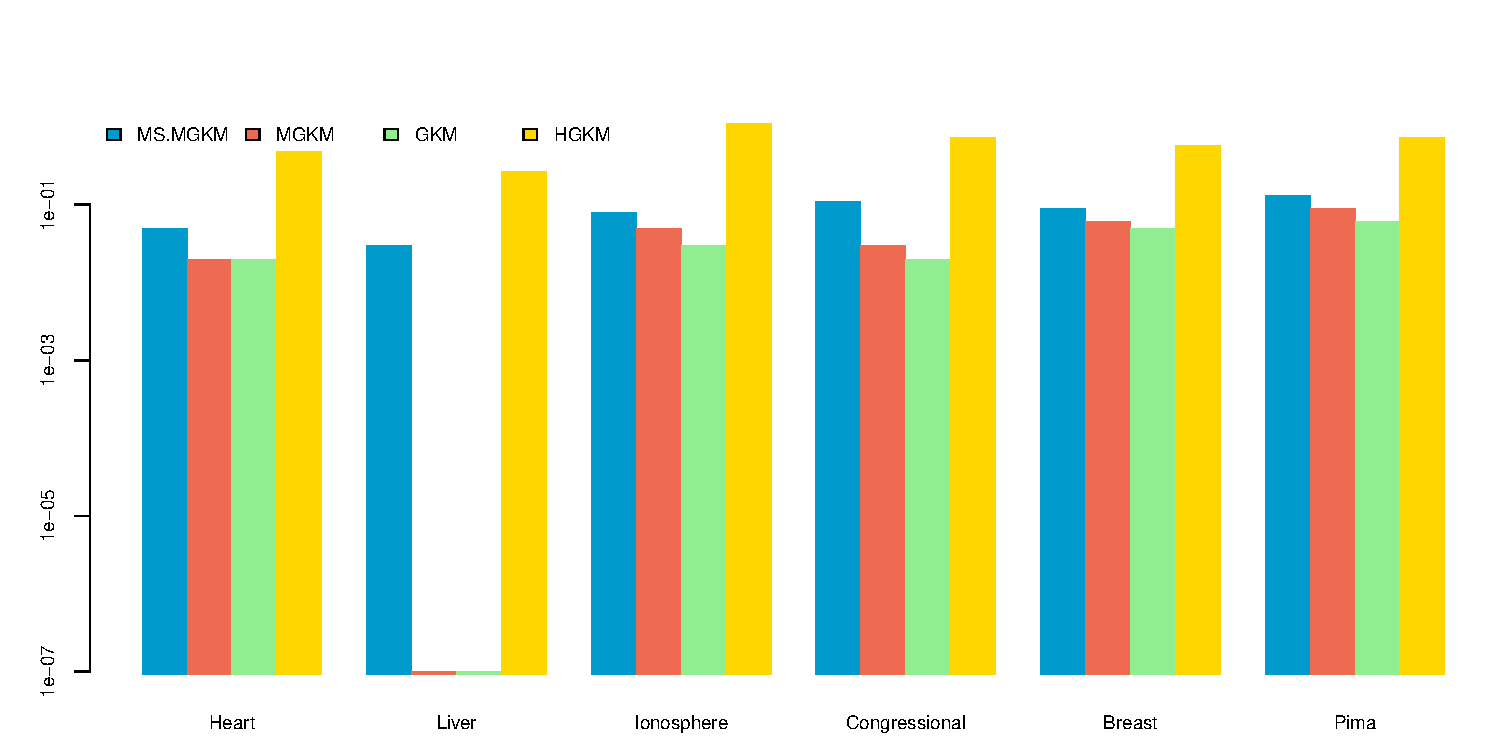
\includegraphics[width=1\textwidth]{img/sizeA2-2}}
\subfigure[$m$ = 10]{\label{fig:sizeA2-10}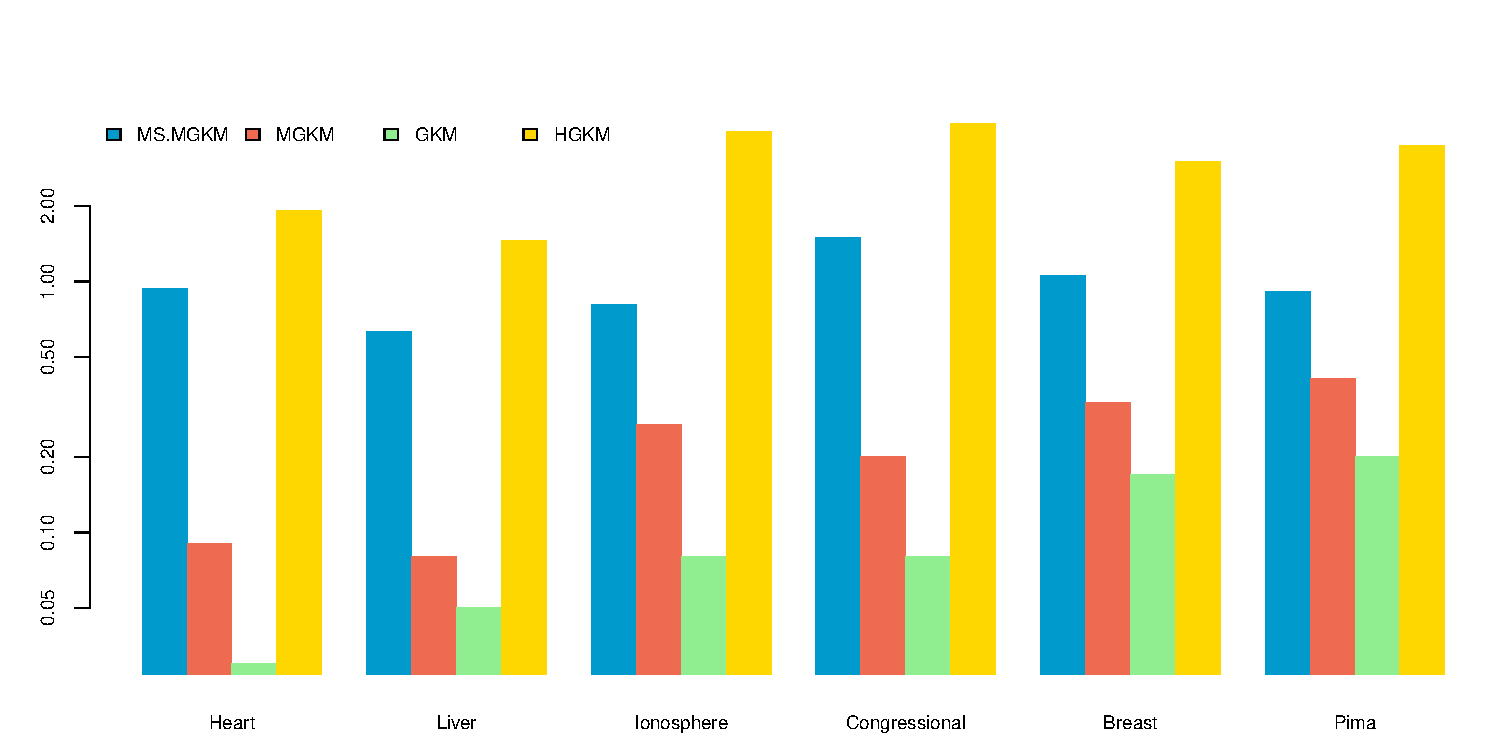
\includegraphics[width=1\textwidth]{img/sizeA2-10}}
\subfigure[$m$ = 20]{\label{fig:sizeA2-20}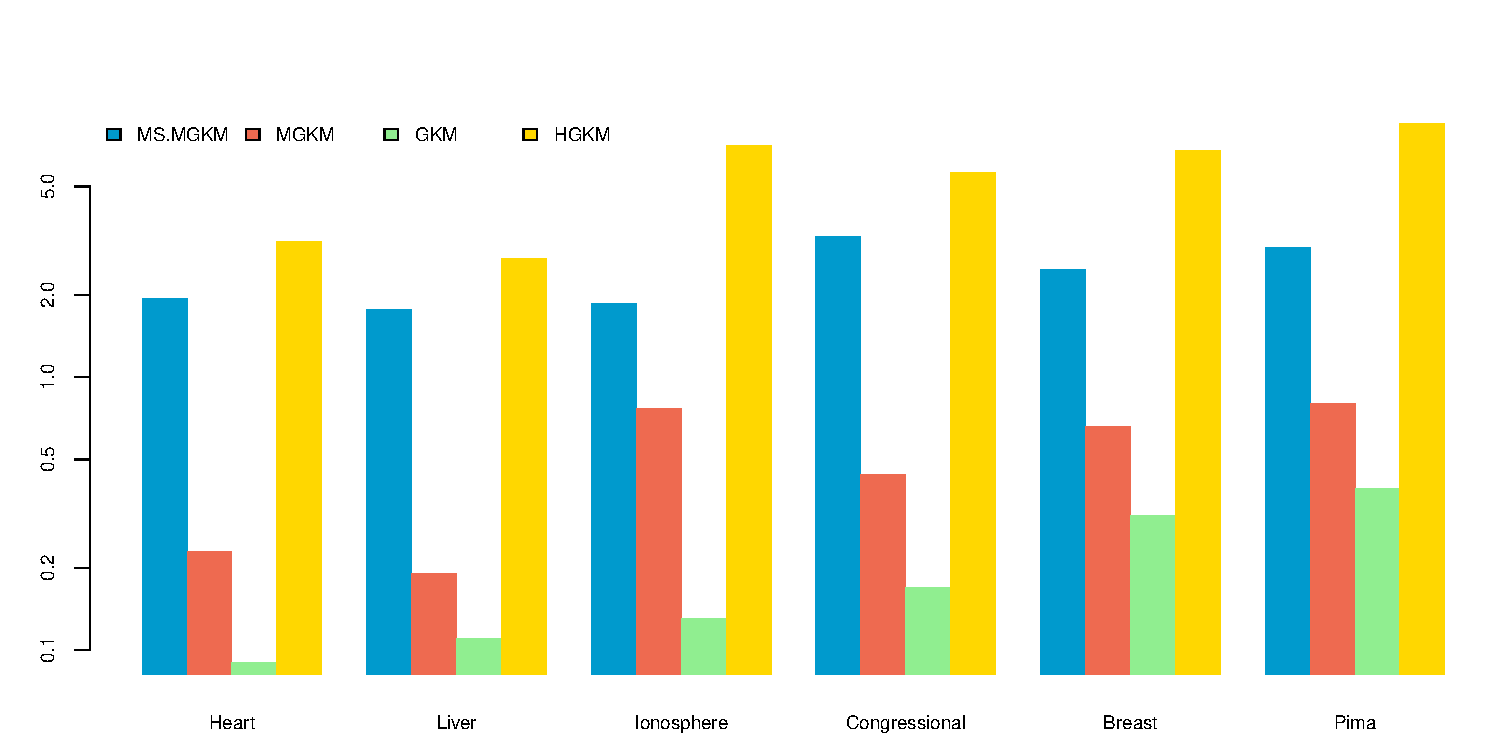
\includegraphics[width=1\textwidth]{img/sizeA2-20}}
\caption{The CPU time of algorithms in Instances A2}
\label{fig:sizeA2}
\end{figure}

\begin{figure}[H]
\centering
\subfigure[$m$ = 2]{\label{fig:sizeB-2}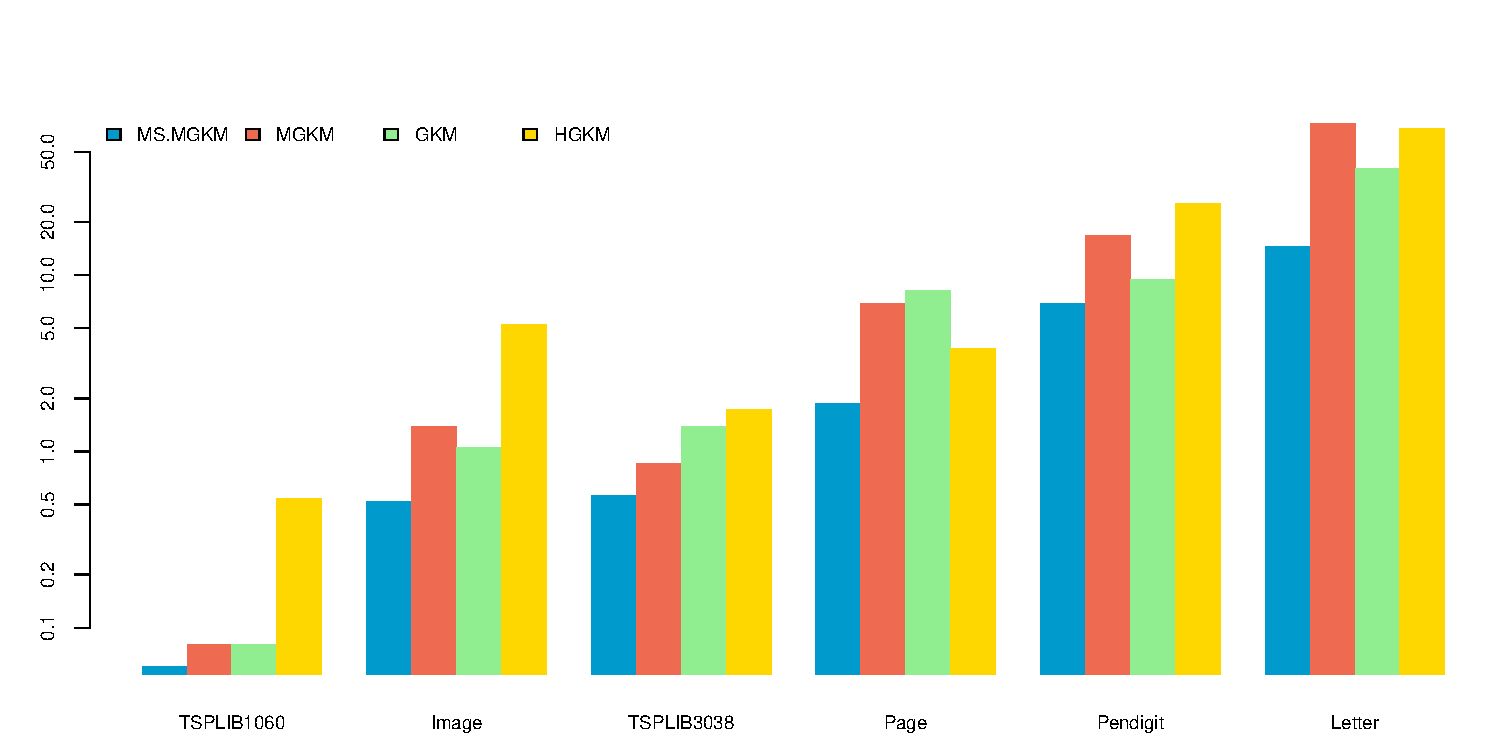
\includegraphics[width=1\textwidth]{img/sizeB-2}}
\subfigure[$m$ = 10]{\label{fig:sizeB-10}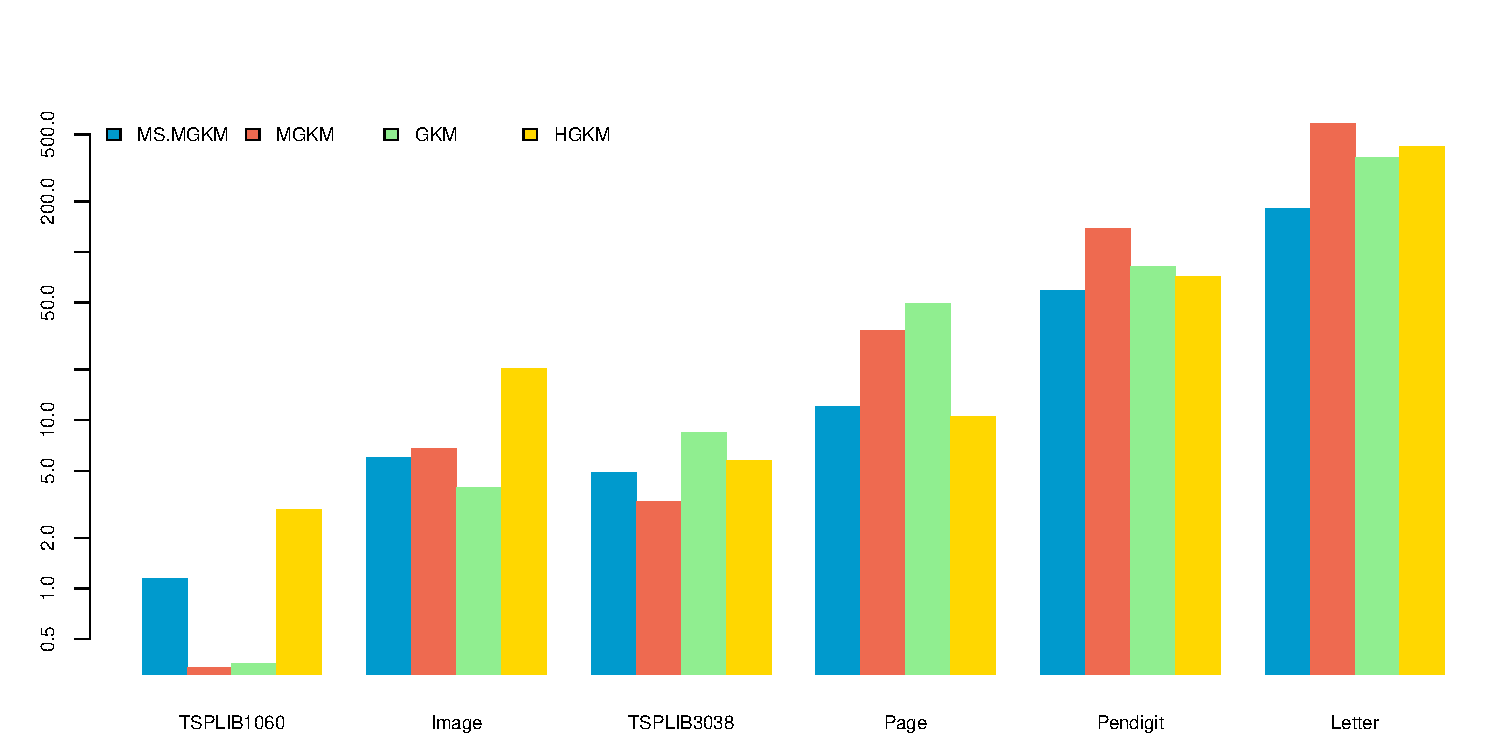
\includegraphics[width=1\textwidth]{img/sizeB-10}}
\subfigure[$m$ = 20]{\label{fig:sizeB-20}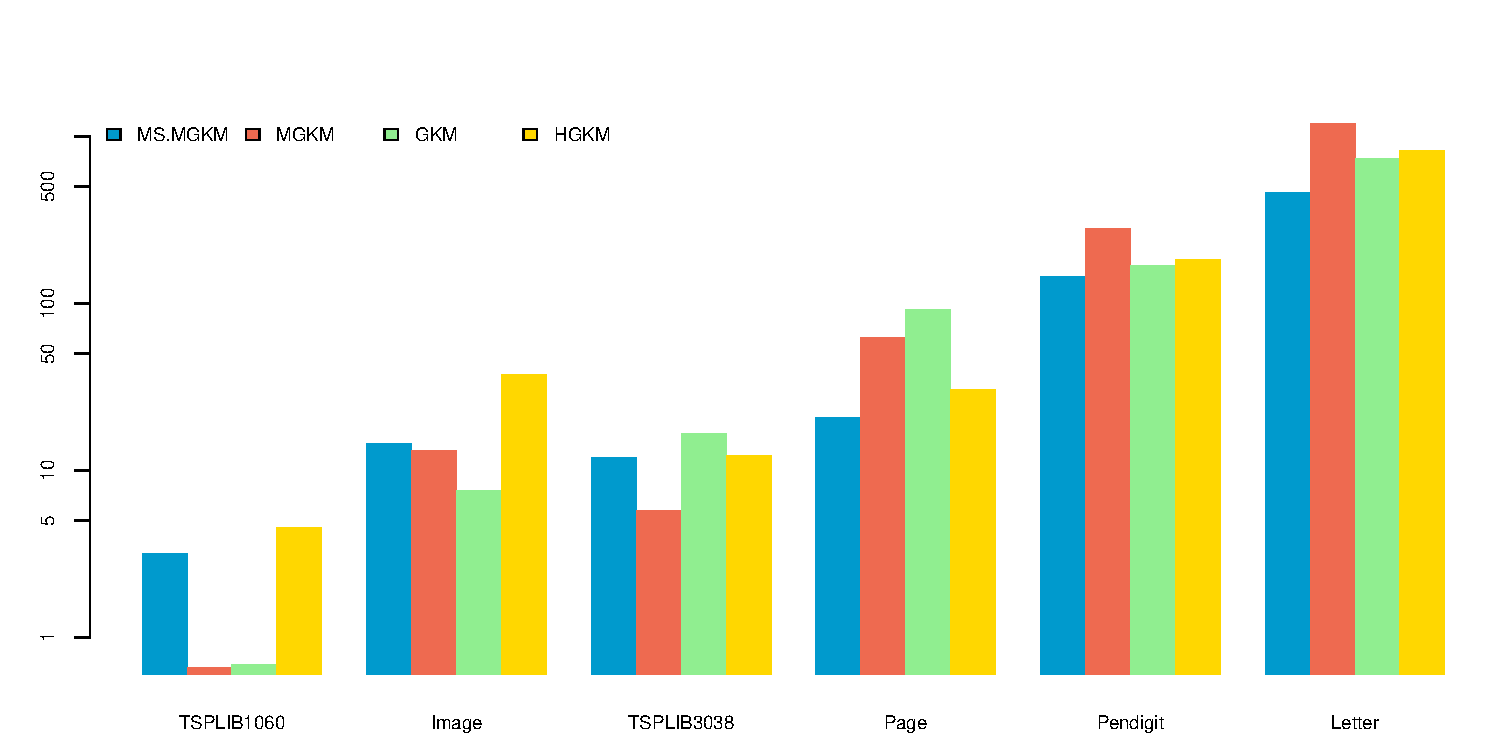
\includegraphics[width=1\textwidth]{img/sizeB-20}}
\caption{The CPU time of algorithms in Instances B}
\label{fig:sizeB}
\end{figure}

\begin{figure}[H]
\centering
\subfigure[$m$ = 2]{\label{fig:sizeC-2}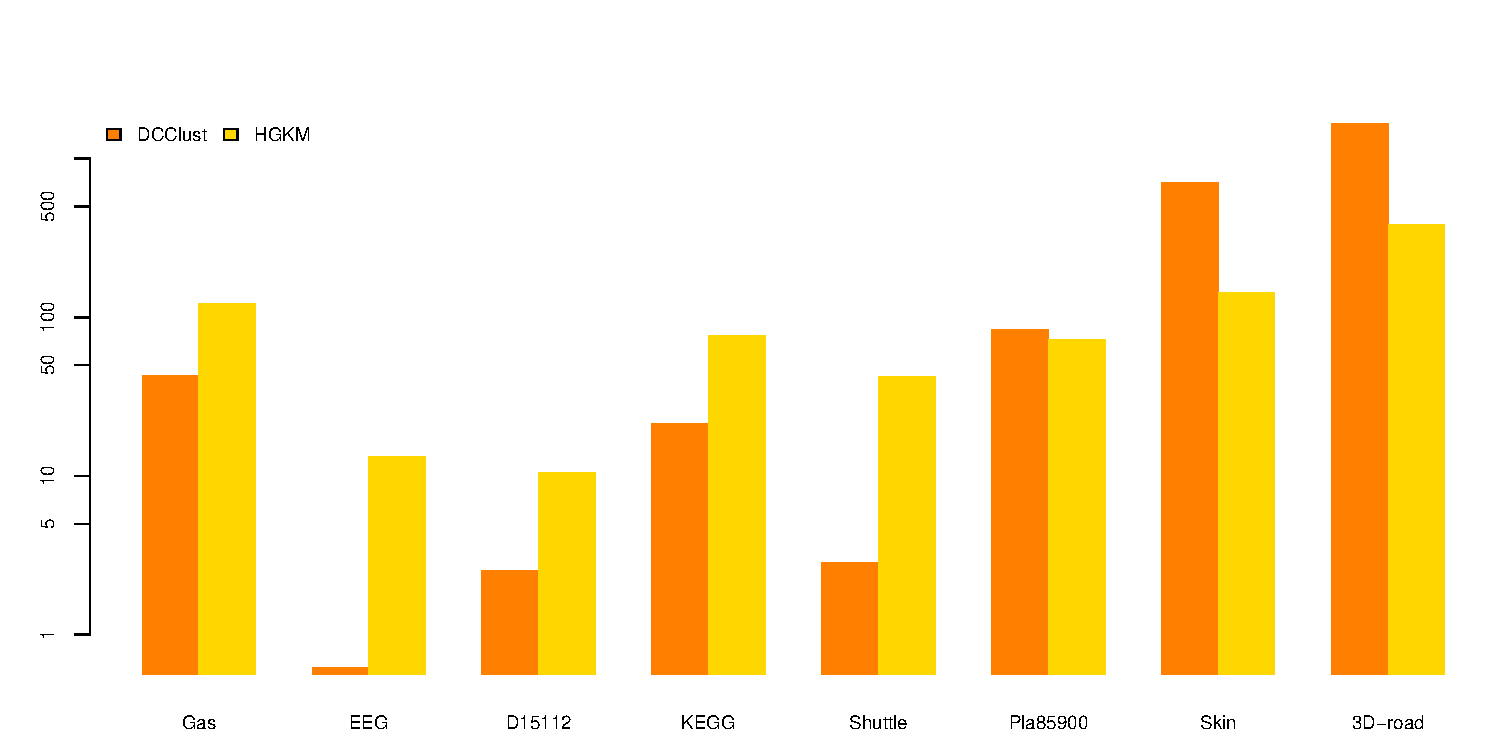
\includegraphics[width=1\textwidth]{img/sizeC-2}}
\subfigure[$m$ = 10]{\label{fig:sizeC-10}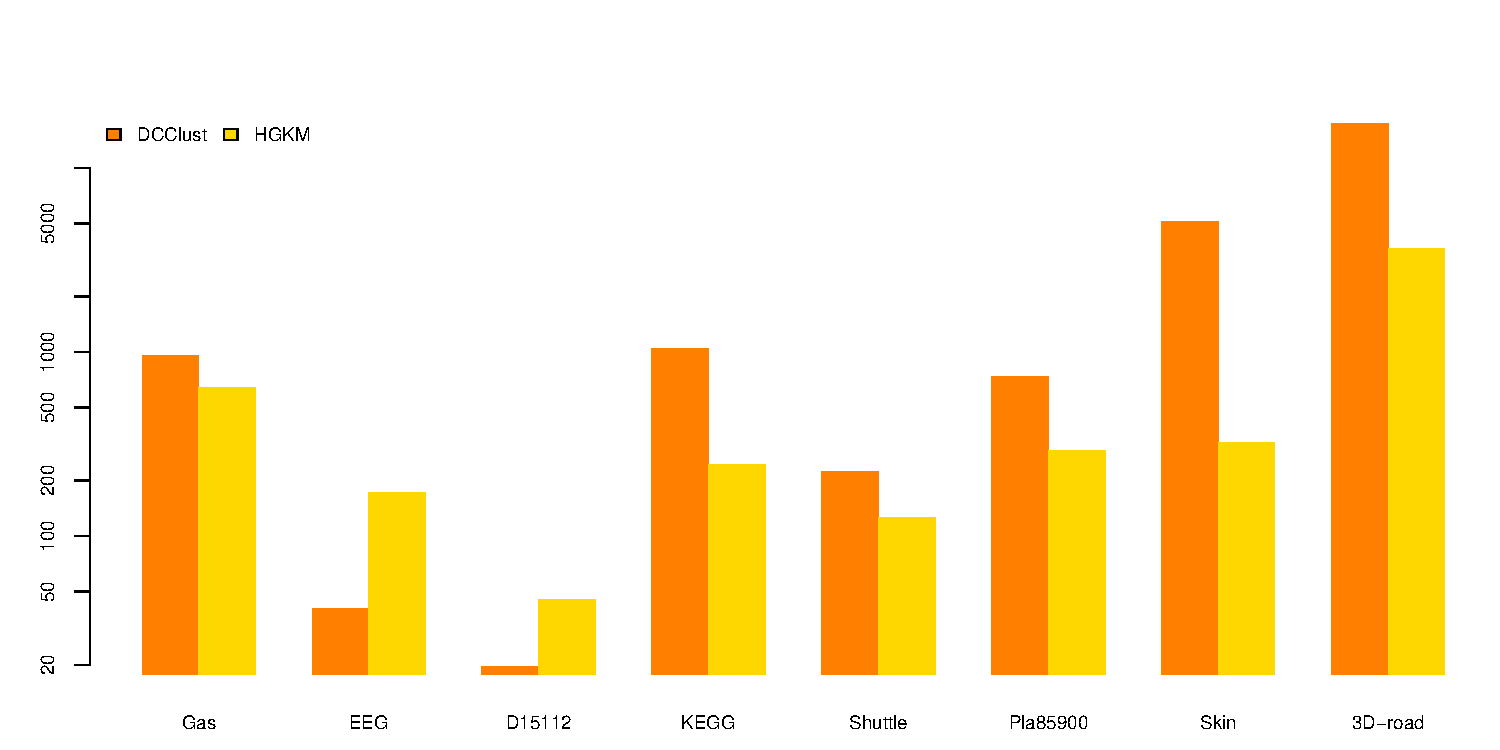
\includegraphics[width=1\textwidth]{img/sizeC-10}}
\subfigure[$m$ = 20]{\label{fig:sizeC-20}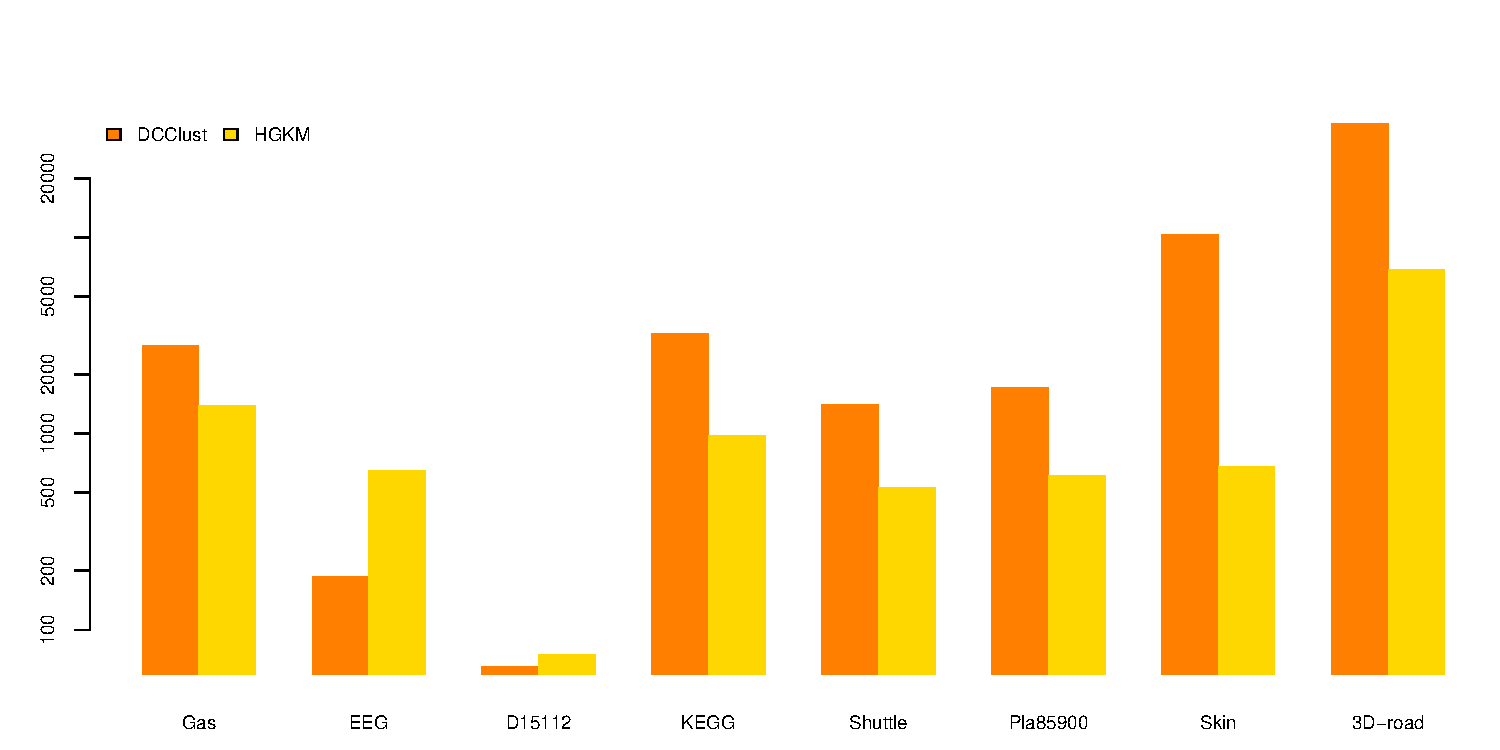
\includegraphics[width=1\textwidth]{img/sizeC-20}}
\caption{The CPU time of algorithms in Instances C}
\label{fig:sizeC}
\end{figure}

\subsection{Components}
\label{sec:components}
In order to understand the contribution of components in the performance of HGKM, we performed some experiments by removing two important operators at a time: crossover and mutation. For comparison purposes, table \ref{components-table} reports the average error with respect to the best known solution in three scenarios: i) complete HGKM with all components ($E_{avg}$), ii) HGKM without mutation ($E_{avg}$ -M) and iii) HGKM without crossover ($E_{avg}$ -C).

\begin{table}[H]
\centering
\begin{tabular}{@{}lccccccccc@{}}
\toprule
Instances A2 &      &       &      &       &       &       &       &       &       \\ \midrule
m            & 2    & 5     & 10   & 15    & 20    & 25    & 30    & 40    & 50    \\
$E_{avg}$    & 0.00 & -0.02 & 0.94 & -0.82 & -1.26 & -1.48 & -1.51 & -1.64 & -1.78 \\
$E_{avg}$ -M   & 0.00 & 0.45  & 3.67 & 3.75  & 5.20  & 6.21  & 6.03  & 4.80  & 3.93  \\
$E_{avg}$ -C   & 0.00 & -0.02 & 0.95 & -0.61 & -0.85 & -0.82 & -0.59 & -0.26 & 0.26  \\ \bottomrule
\end{tabular}
\caption{HGKM performance in different scenarios: with all components, without mutation and without crossover.}
\label{components}
\end{table}

The role of mutation and crossover is very important on finding good solutions. Particularly, for the case where we have HGKM without mutation, it does not find (in average) a solution better than the best known so far, while in the two other scenarios (complete HGKM and HGKM without crossover), it has a significantly better performance. Additionally, the complete HGKM algorithm performs better than the HGKM without crossover, especially when $m$ increases, indicating that the crossover is an essential operator when dealing with more complex clustering tasks.

\noindent [TO-DO] the exact times for the DCClust and MS-DCA algorithms in group C of instances

%\noindent [TO-DO] analysis on number of features -- our algorithm seems to be fast when $d$ is small in small/medium instances (tsplib for example) but also when $d$ is large in large instances (gas sensor for example)
  % -*- coding: utf-8; -*-
\chapter{Conclusions and Future work}

-- Review 1: About the problem and the model-oriented approach to solve clustering.
In this dissertation the MSSC problem was ...

-- Review 2: About the method (meta-heuristic).
In this work a meta-heuristic was proposed to solve the MSSC problem ...

-- Mutation: The role of mutation in diversification and its importance to final results

-- Results (cost): The proposed method outperformed the best current literature results for all considered sets of benchmark
instances in terms of solution quality for MSSC

-- Results (time): In terms of time, the proposed method outperformed some state-of-the-art algorithms in large instances

-- The proposed meta-heuristic is easy to understand and implement

-- Future work: Solve different objectives in clustering. As we tackle the clustering problem from an optimization perspective through a meta-heuristic, we can elaborate a neighbourhood structure that is general enough to deal with different models
  \arial
  \bibliography{reference}
  \normalfont
  %% -*- coding: utf-8; -*-

\appendix
\chapter{Artigo da tese publicado em periódico}

O método de segmentação Crescimento de Regiões Modificado mostrado neste
trabalho rendeu uma publicação no periódico \textit{Minerals
  Engineering}. Esta publicação serve como requisito parcial para
obtenção do título de Doutor pelo Programa de Pós-graduação em
Engenharia de Materiais e de Processos Químicos e Metalúrgicos da
PUC-Rio. É por isto que esta publicação será anexada à continuação desta
página.



\end{document}
